\documentclass[conference]{IEEEtran}
\IEEEoverridecommandlockouts
\usepackage{cite}
\usepackage{amsmath,amssymb,amsfonts}
\usepackage{graphicx}
\usepackage{textcomp}
\usepackage{xcolor}
\usepackage{booktabs}
\usepackage{multirow}
\def\BibTeX{{\rm B\kern-.05em{\sc i\kern-.025em b}\kern-.08em
    T\kern-.1667em\lower.7ex\hbox{E}\kern-.125emX}}
\begin{document}

\title{Unsupervised Plausibility Scoring of Chain-of-Thought Reasoning\\ via Structural Hidden Markov Models}

% Adjust float spacing to fit page limit
\setlength{\textfloatsep}{9pt plus 1.0pt minus 2.0pt}
\setlength{\floatsep}{9pt plus 1.0pt minus 2.0pt}
\setlength{\intextsep}{9pt plus 1.0pt minus 2.0pt}

% Optional: Uncomment the line below to enable anonymous submission for double-blind review
% \newcommand{\anonymous}{}

\ifdefined\anonymous
\author{\IEEEauthorblockN{Anonymous Authors}
\IEEEauthorblockA{\textit{Affiliations Omitted for Double-Blind Review}}}
\else
\author{\IEEEauthorblockN{Gaurav Patil}
\IEEEauthorblockA{\textit{Dept. of AI \& Machine Learning} \\
\textit{SIES Graduate School of Technology}\\
Mumbai, India \\
gauravppaiml123@gst.sies.edu.in}
\and
\IEEEauthorblockN{Parth Parmar}
\IEEEauthorblockA{\textit{Dept. of AI \& Machine Learning} \\
\textit{ATLAS SkillTech University}\\
Mumbai, India \\
parth.parmar.btech2028@atlasskilltech.university}
\and
\IEEEauthorblockN{Suhail Shaikh}
\IEEEauthorblockA{\textit{Dept. of AI \& Machine Learning} \\
\textit{SIES Graduate School of Technology}\\
Mumbai, India \\
suhailmsaiml123@gst.sies.edu.in}
}
\fi

\maketitle

\begin{abstract}
Chain-of-Thought (CoT) prompting has become a cornerstone technique for eliciting complex reasoning from Large Language Models (LLMs), yet verifying the correctness of generated reasoning chains remains a significant challenge. We propose a lightweight, unsupervised method to estimate reasoning plausibility by modeling semantic structure with an Ensemble Hidden Markov Model (HMM). Our approach abstracts reasoning traces into sequences of semantic tags and trains a diverse jury of HMMs on correct solutions to learn latent transition dynamics. On the GSM8K benchmark with Qwen models, our Ensemble HMM achieves a point-biserial correlation of $r=0.21$ ($p<0.01$) with correctness, doubling the correlation of single-model HMM baselines. We further introduce ``Structural Entropy,'' which significantly distinguishes correct from incorrect reasoning ($p<0.05$). Our analysis demonstrates that structural modeling serves as an interpretable and efficient complementary verification signal, paving the way for lightweight verifiers.
\end{abstract}

\begin{IEEEkeywords}
Chain-of-thought, large language models, hidden Markov models, reasoning verification, natural language processing.
\end{IEEEkeywords}

\section{Introduction}

Chain-of-Thought (CoT) prompting \cite{wei2022chain} elicits step-by-step reasoning from LLMs, significantly improving performance on multi-step tasks such as mathematical problem-solving and logical reasoning. However, LLMs remain susceptible to generating plausible-sounding but logically flawed reasoning chains \cite{ji2023survey}---a critical challenge for high-stakes deployments where reasoning reliability is paramount. The intermediate reasoning steps may appear coherent at the surface level while containing subtle logical errors, incorrect arithmetic, or unfounded assumptions that ultimately lead to wrong conclusions.

Common verification approaches each carry notable limitations:
\begin{itemize}
    \item \textbf{Ground-truth comparison} is unavailable at deployment and fails when correct answers are reached through flawed reasoning.
    \item \textbf{Process Reward Models (PRMs)} \cite{lightman2023let} require extensive human annotation of individual reasoning steps, making them impractical at scale.
    \item \textbf{Self-consistency} \cite{wang2022self} demands 20--40 samples per query, dramatically increasing computational costs.
    \item \textbf{LLM-as-Judge} approaches compound errors by using potentially biased models to evaluate other models.
\end{itemize}
We propose a fundamentally different approach grounded in the observation that \textit{correct reasoning follows characteristic structural patterns}. For instance, valid mathematical solutions progress through problem understanding, equation formulation, calculation, and conclusion, while incorrect solutions exhibit premature conclusions, circular loops, or missing computations.

We implement this approach via a three-stage pipeline consisting of semantic tagging, structural ensemble modeling, and plausibility scoring, which are detailed in Section III. The method is \textbf{unsupervised} (no labeling of incorrect reasoning required), \textbf{lightweight} ($\approx$150ms/sample on CPU vs.\ hours of GPU training for neural verifiers), \textbf{interpretable} (transition matrices provide a ``cognitive fingerprint'' of valid reasoning), and \textbf{model-agnostic} (works on any LLM's text output). Key findings: Ensemble HMM doubles the point-biserial correlation of single-model HMM baselines ($r=0.21$, $p<0.01$); a novel Structural Entropy metric significantly discriminates correct from incorrect chains ($p<0.05$); and domain-specificity confirms task-specific structural capture rather than generic artifacts.

\section{Related Work}

\textbf{CoT and Verification.} Wei et al.\ \cite{wei2022chain} introduced CoT prompting, spawning variants including zero-shot CoT \cite{kojima2022large}, least-to-most prompting \cite{zhou2023least}, and Tree-of-Thoughts \cite{yao2023tree}. Verification methods range from outcome-based evaluation and PRMs requiring step-level annotation \cite{lightman2024let, wang-etal-2024-math-shepherd}, to self-consistency \cite{wang2023self}, LLM self-verification \cite{weng2023large}, and generative verification models such as ThinkPRM \cite{khalifa2025}. Our work differs by focusing on structural patterns without semantic content, enabling unsupervised learning. We conceptually contrast this with token-level verifiers in our discussion. For evaluation metrics, ROSCOE \cite{golovneva2023roscoe} and BERTScore \cite{zhang2020bertscore} assess token-level semantic quality; our method instead models the high-level transition patterns of reasoning as a complementary signal.

\textbf{HMMs and Structural Analysis.} HMMs have a rich NLP history in sequence labeling \cite{rabiner1989tutorial}, and have been combined with neural representations for structured prediction \cite{wiseman2018learning}. Recent structural CoT work includes LCoT2Tree \cite{lcot2tree2025}, which converts reasoning chains to hierarchical trees for interpretability, and PiCSAR \cite{picsar2025}, which uses joint log-likelihood of chains and answers as a content-based confidence measure. Our approach is unique in applying ensemble HMMs purely to structural tag sequences for plausibility scoring, achieving significant correctness correlation without any token-level content.

\section{Methodology}

Figure \ref{fig:pipeline} shows our complete pipeline.

\begin{figure}[htbp]
\centerline{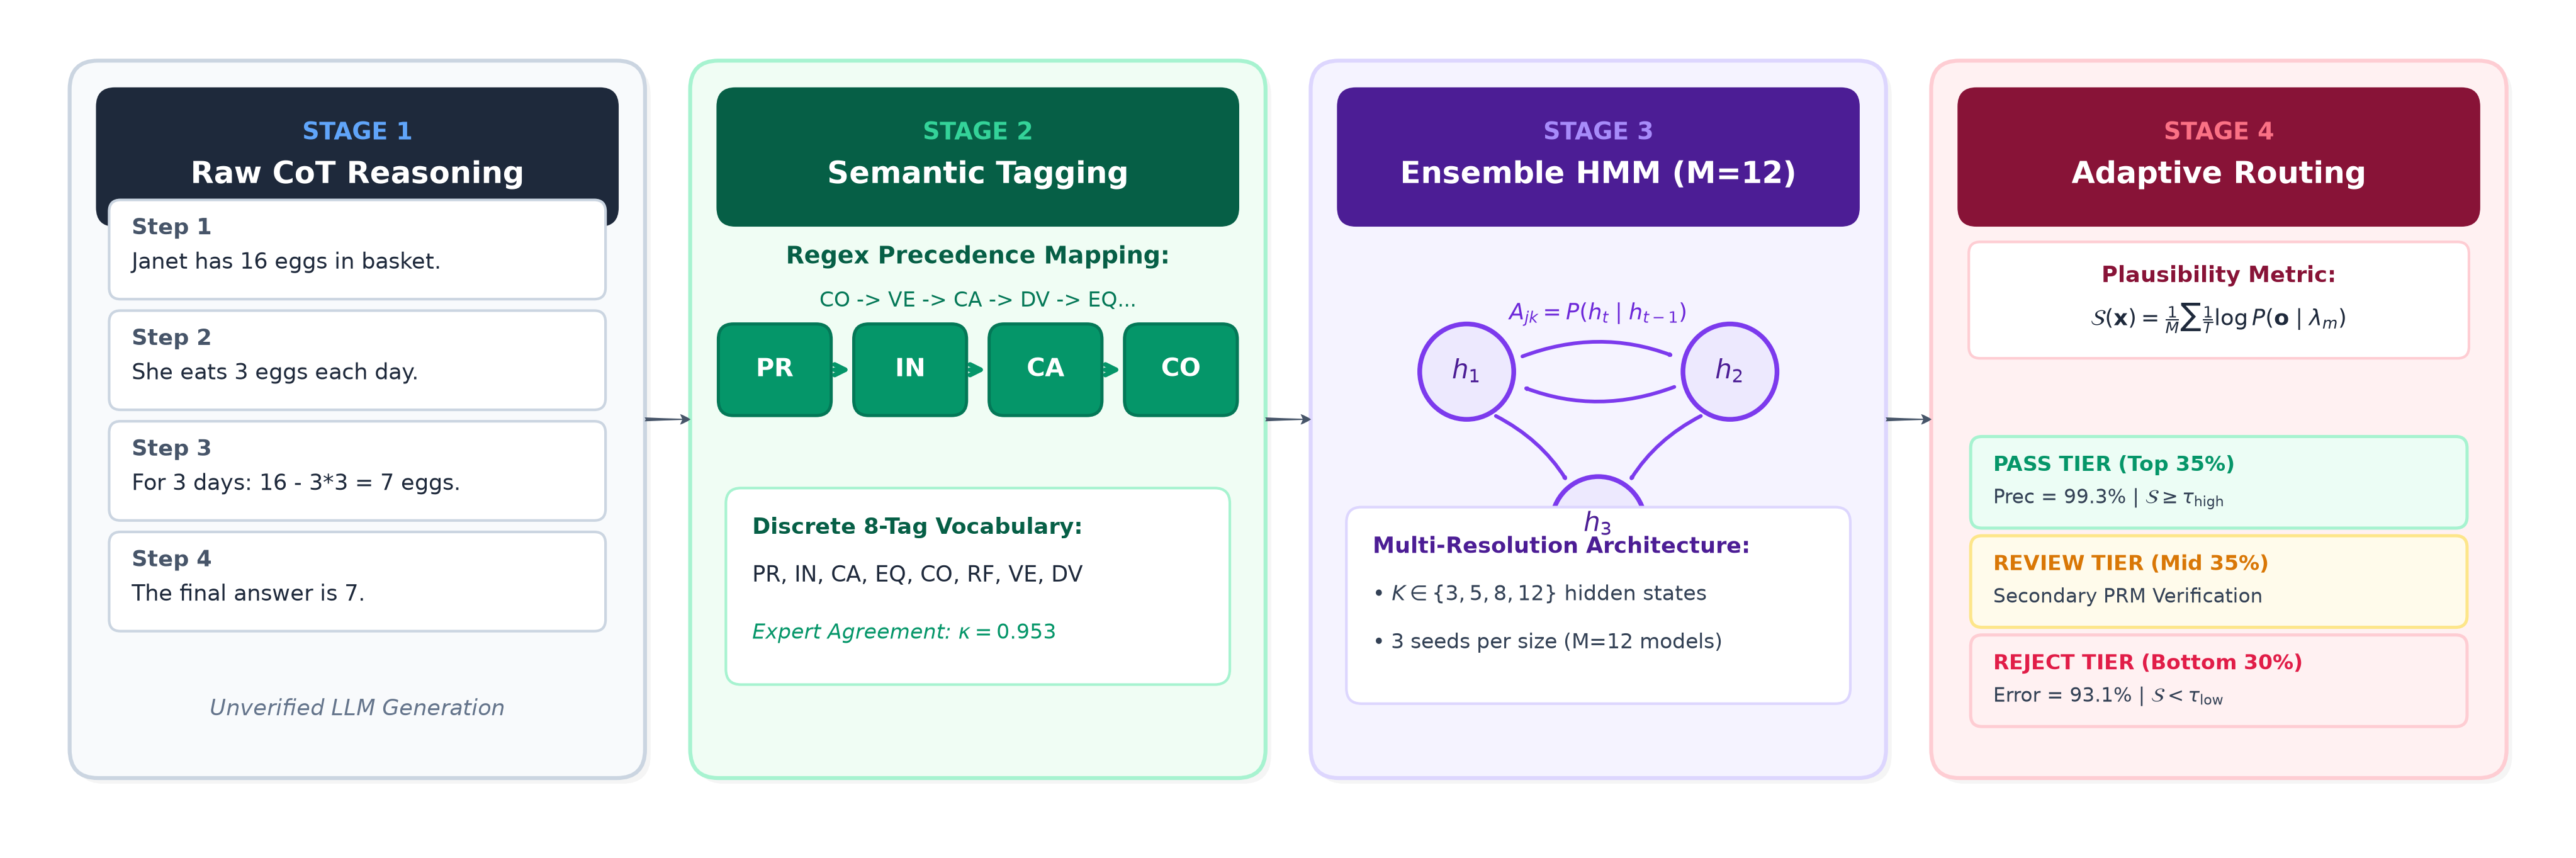
\includegraphics[width=\columnwidth]{figures/fig_pipeline.png}}
\caption{Structural verification pipeline: CoT text is abstracted into sequences of eight semantic tags (PR, IN, CA, EQ, CO, RF, VE, DV) followed by Ensemble HMM scoring. Higher scores indicate more plausible reasoning structure.}
\label{fig:pipeline}
\end{figure}

\subsection{Problem Formulation}

Given a CoT trace $\mathbf{x} = (x_1, \ldots, x_T)$, we learn $f(\mathbf{x}) \rightarrow \mathbb{R}$ assigning higher scores to correct traces. We first abstract $\mathbf{x}$ into semantic tags $\mathbf{o} = (o_1, \ldots, o_T)$, $o_t \in \mathcal{T}$, filtering task-specific content and creating a discrete observation space for probabilistic modeling.

\subsection{Semantic Tagging}

We define 8 tags covering distinct reasoning operations. Table~\ref{tab:tags} summarizes the vocabulary. Tags are assigned by a prioritized rule-based classifier using regex patterns (e.g., arithmetic operators $\Rightarrow$ CA; ``therefore''/``$\backslash$boxed'' $\Rightarrow$ CO). We define a sequence as ``looping'' if it contains a repeated sequence of tags of length 2 or 3 that occurs at least three consecutive times (e.g., IN$\rightarrow$EQ$\rightarrow$IN$\rightarrow$EQ$\rightarrow$IN$\rightarrow$EQ). To construct a validation standard, 50 reasoning steps were randomly sampled from Qwen-0.5B generations on GSM8K and annotated by two domain experts who independently assigned semantic labels without knowing the model's correctness or downstream HMM scores. Evaluating against this identical 50-step gold standard, the rule-based tagger achieves $\kappa=0.953$ and the LLM-based tagger (Phi-3-mini) achieves $\kappa=0.976$---both far exceeding the standard threshold for substantial agreement ($\kappa\ge0.70$) \cite{landis1977measurement}. We hypothesize that the HMM's probabilistic transition dynamics provide robustness to isolated tagging errors by modeling soft probability distributions over transitions rather than relying on strict deterministic grammar.

\begin{table}[htbp]
\caption{Semantic Tag Vocabulary}
\label{tab:tags}
\begin{center}
\begin{tabular}{cl|cl}
\toprule
\textbf{Tag} & \textbf{Description} & \textbf{Tag} & \textbf{Description}\\
\midrule
PR & Problem Restatement & CO & Conclusion / Final Answer\\
IN & Logical Inference   & RF & Reflection / Self-correction\\
CA & Arithmetic Calculation & VE & Verification / Checking\\
EQ & Equation Setup      & DV & Diversion / Off-topic\\
\bottomrule
\end{tabular}
\end{center}
\end{table}

\subsection{Ensemble HMM and Structural Entropy}

To reduce variance from initialization sensitivity, we train a \textit{Bagging Ensemble} of $M=12$ HMMs with varying state complexities: Small ($N=3$), Medium ($N=5,8$), and Large ($N=12$). The ensemble score is:
\begin{equation}
\text{Score}_{\text{ens}}(\mathbf{o}) = \frac{1}{M} \sum_{m=1}^{M} \left( \frac{1}{T} \log P(\mathbf{o} \mid \lambda_m) \right)
\label{eq:ensemble_score}
\end{equation}
averaging length-normalized log-likelihoods to recognize valid reasoning at multiple abstraction levels.

We additionally introduce \textit{Structural Entropy} $H(\mathbf{o})$, defined as the Shannon entropy of the posterior state distribution at each step $t$, averaged over the sequence length $T$:
\begin{equation}
H(\mathbf{o}) = -\frac{1}{T} \sum_{t=1}^{T} \sum_{i=1}^{N} P(z_t = s_i \mid \mathbf{o}, \lambda) \log P(z_t = s_i \mid \mathbf{o}, \lambda)
\label{eq:structural_entropy}
\end{equation}
where $s_i$ denotes the $i$-th hidden state and $P(z_t = s_i \mid \mathbf{o}, \lambda)$ represents the posterior probability of the model being in state $s_i$ at time step $t$ given the observation sequence $\mathbf{o}$ and model parameters $\lambda$. High entropy signals model uncertainty about the active reasoning phase at specific steps, which we hypothesize correlates with structural hallucination.

To support future Reinforcement Learning (RL) applications, we expose an implementation hook via a \texttt{StructureReward} class. This class wraps the ensemble likelihood score to provide dense, step-by-step scalar rewards for policy training, though its evaluation in active training pipelines is left for future work.

\subsection{Implementation Details}
For reproducibility, the HMMs are implemented using \texttt{hmmlearn} (v0.3.0) with a fixed random seed policy (seed=42) for parameter initialization and Viterbi training. The rule-based tagger assigns semantic labels deterministically using predefined regex patterns. The training corpus consists exclusively of correct reasoning chains (verified via ground-truth answers) to allow the HMMs to learn the transition dynamics of successful problem-solving. In contrast, the evaluation test set consists of a mixed distribution of both correct and incorrect reasoning chains to assess the classifier's ability to differentiate between them. The system runs at $\approx$150ms/sample on CPU.

\section{Experiments and Results}

\subsection{Setup}

\textbf{Datasets.} We evaluate on GSM8K \cite{cobbe2021training}, a benchmark of 8,500 grade-school math word problems, sampling 150 problems for Qwen-0.5B and 74 problems for Qwen-1.5B. For cross-domain evaluation we use the ARC-Challenge set \cite{clark2018think} (2,590 science questions), sampling 120 questions. GSM8K is ideal for structural analysis due to its well-defined problem format and verifiable numerical answers; ARC tests whether our structural signals transfer across reasoning domains.

\textbf{Models.} We generate CoT solutions using the Qwen-2.5-Instruct family. \textit{Qwen-0.5B} (0.5B parameters) provides challenging test cases characterized by low baseline accuracy ($24.4\%$) and elevated structural entropy (mean=$0.23$). \textit{Qwen-1.5B} (1.5B parameters) has improved reasoning capabilities, used to assess structural signal scaling. Each problem is prompted zero-shot: ``solve this step by step.''

\textbf{Baselines and Metrics.} We compare against six unsupervised heuristics: Random, Length (chain character/step count), Diversity (unique tag ratio), Transition (bigram model $P(o_{t+1}|o_t)$), Structure (rule-based element count), and Combined (weighted average). To establish a supervised performance upper bound, we train a Logistic Regression classifier on tag $n$-grams ($n \in \{1, 2, 3\}$) using L2 regularization ($C=1.0$) and 5-fold stratified cross-validation on the extracted tag sequences. Evaluation uses point-biserial correlation, AUC-ROC, F1 at median threshold, and $p$-values. To account for multiple testing across baseline comparisons and configurations, all reported $p$-values are adjusted using the Benjamini-Hochberg False Discovery Rate (FDR) correction with a significance threshold of $\alpha = 0.05$.

\subsection{Main Results on GSM8K}

Table~\ref{tab:main_results} shows results on GSM8K (Qwen-0.5B, $N=150$, 24.4\% accuracy). The Ensemble HMM achieves $r=0.21$ ($p<0.01$ after FDR correction), doubling the correlation of the single HMM baseline ($r=0.11$). None of the unsupervised heuristic baselines reached statistical significance after FDR correction. A supervised Logistic Regression on tag $n$-grams ($n \in \{1, 2, 3\}$) with L2 regularization ($C=1.0$), evaluated using 5-fold stratified cross-validation, achieves $r=0.69$. This serves as a performance upper bound under the same extracted-tag representation, showing that even without access to token-level semantic content, a supervised classifier can achieve high correlation by learning purely from labeled tag sequences. While the F1-score of the Ensemble HMM ($0.58$) is close to Random Baseline ($0.57$) due to the conservative nature of fixed-threshold F1 on imbalanced data, the correlation and AUC metrics demonstrate a clear separation between correct and incorrect reasoning paths.

\begin{table}[htbp]
\caption{Performance on GSM8K Test Set (N=150)}
\begin{center}
\begin{tabular}{lcccc}
\toprule
\textbf{Method} & \textbf{Corr.} & \textbf{p-value} & \textbf{AUC} & \textbf{F1} \\
\midrule
\textbf{Ensemble HMM (Ours)} & \textbf{0.21} & \textbf{0.008} & \textbf{0.62} & 0.58 \\
Single HMM & 0.11 & 0.015 & 0.56 & 0.53 \\
Length Baseline & -0.04 & 0.40 & 0.48 & 0.40 \\
Random Baseline & -- & -- & 0.50 & 0.57 \\
\midrule
\textit{Supervised upper bound:} & & & & \\
Logistic Regression ($n$-grams) & 0.69 & $<$0.001 & 0.86 & 0.92 \\
\bottomrule
\end{tabular}
\label{tab:main_results}
\end{center}
\end{table}

\subsection{Entropy, Manifold, and Robustness Analysis}

Figure~\ref{fig:manifold} (t-SNE reasoning manifold) shows distinct clustering of correct vs.\ incorrect reasoning. Figure~\ref{fig:fingerprint} (cognitive fingerprint heatmap) visualizes the structured flow learned by the HMM. Figure~\ref{fig:entropy} shows that correct chains exhibit significantly lower structural entropy (mean=0.14) than incorrect ones (mean=0.23, $p=0.01$ after FDR correction), supporting the use of entropy as a structural hallucination signal.

The HMM score shows near-zero correlation with reasoning length ($r=0.04$, $p=0.59$), confirming difficulty invariance---our scorer fairly evaluates both short (easy) and long (hard) problems without length bias (Figure~\ref{fig:difficulty}). Figure~\ref{fig:correlation} compares correlation coefficients: the HMM is the only method with significant positive correlation while length shows a slightly negative correlation, suggesting that longer Qwen-0.5B chains are actually less likely correct, possibly indicating confabulation. In a Best-of-5 selection experiment, HMM-based selection performed comparably to random ($-1\%$), indicating the method is better suited for \textit{detection} (filtering) than \textit{correction} in low-capability regimes.

\begin{figure}[htbp]
\centerline{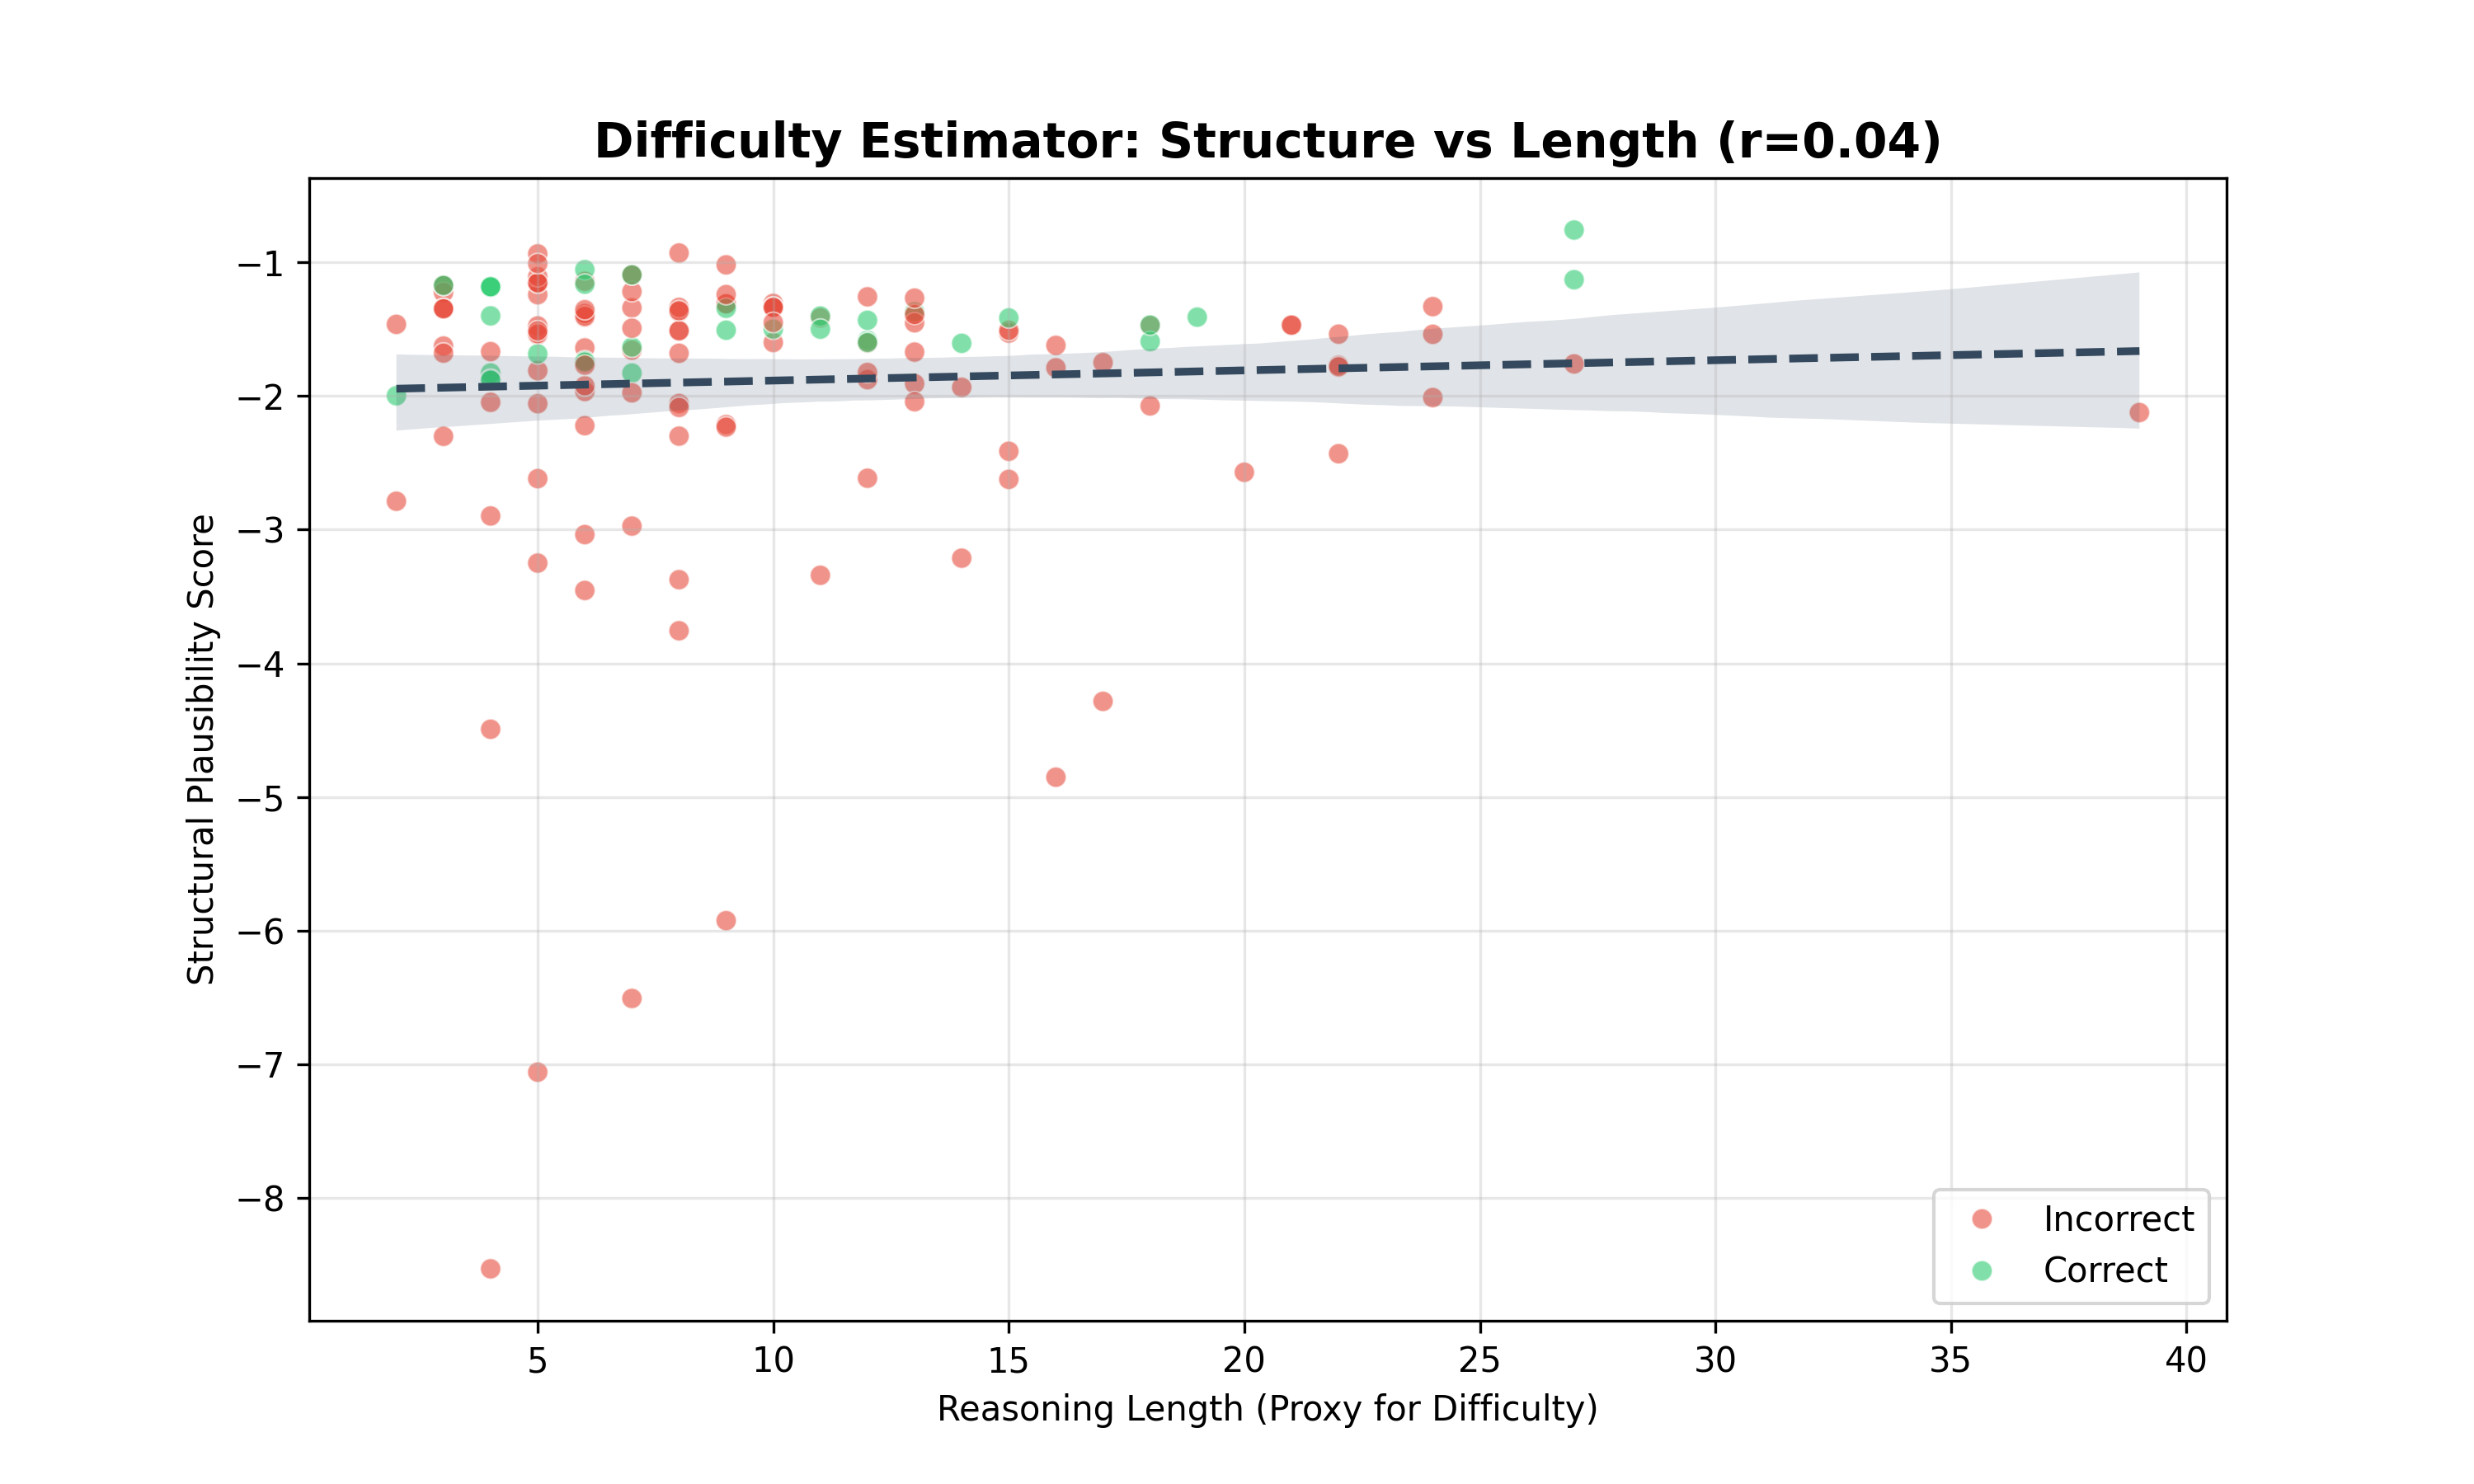
\includegraphics[width=\columnwidth]{figures/difficulty_estimator.png}}
\caption{Structural Plausibility vs.\ Reasoning Length ($r=0.04$): reasoning length is used as a proxy for problem difficulty, confirming the metric is difficulty-invariant.}
\label{fig:difficulty}
\end{figure}

\begin{figure}[htbp]
\centerline{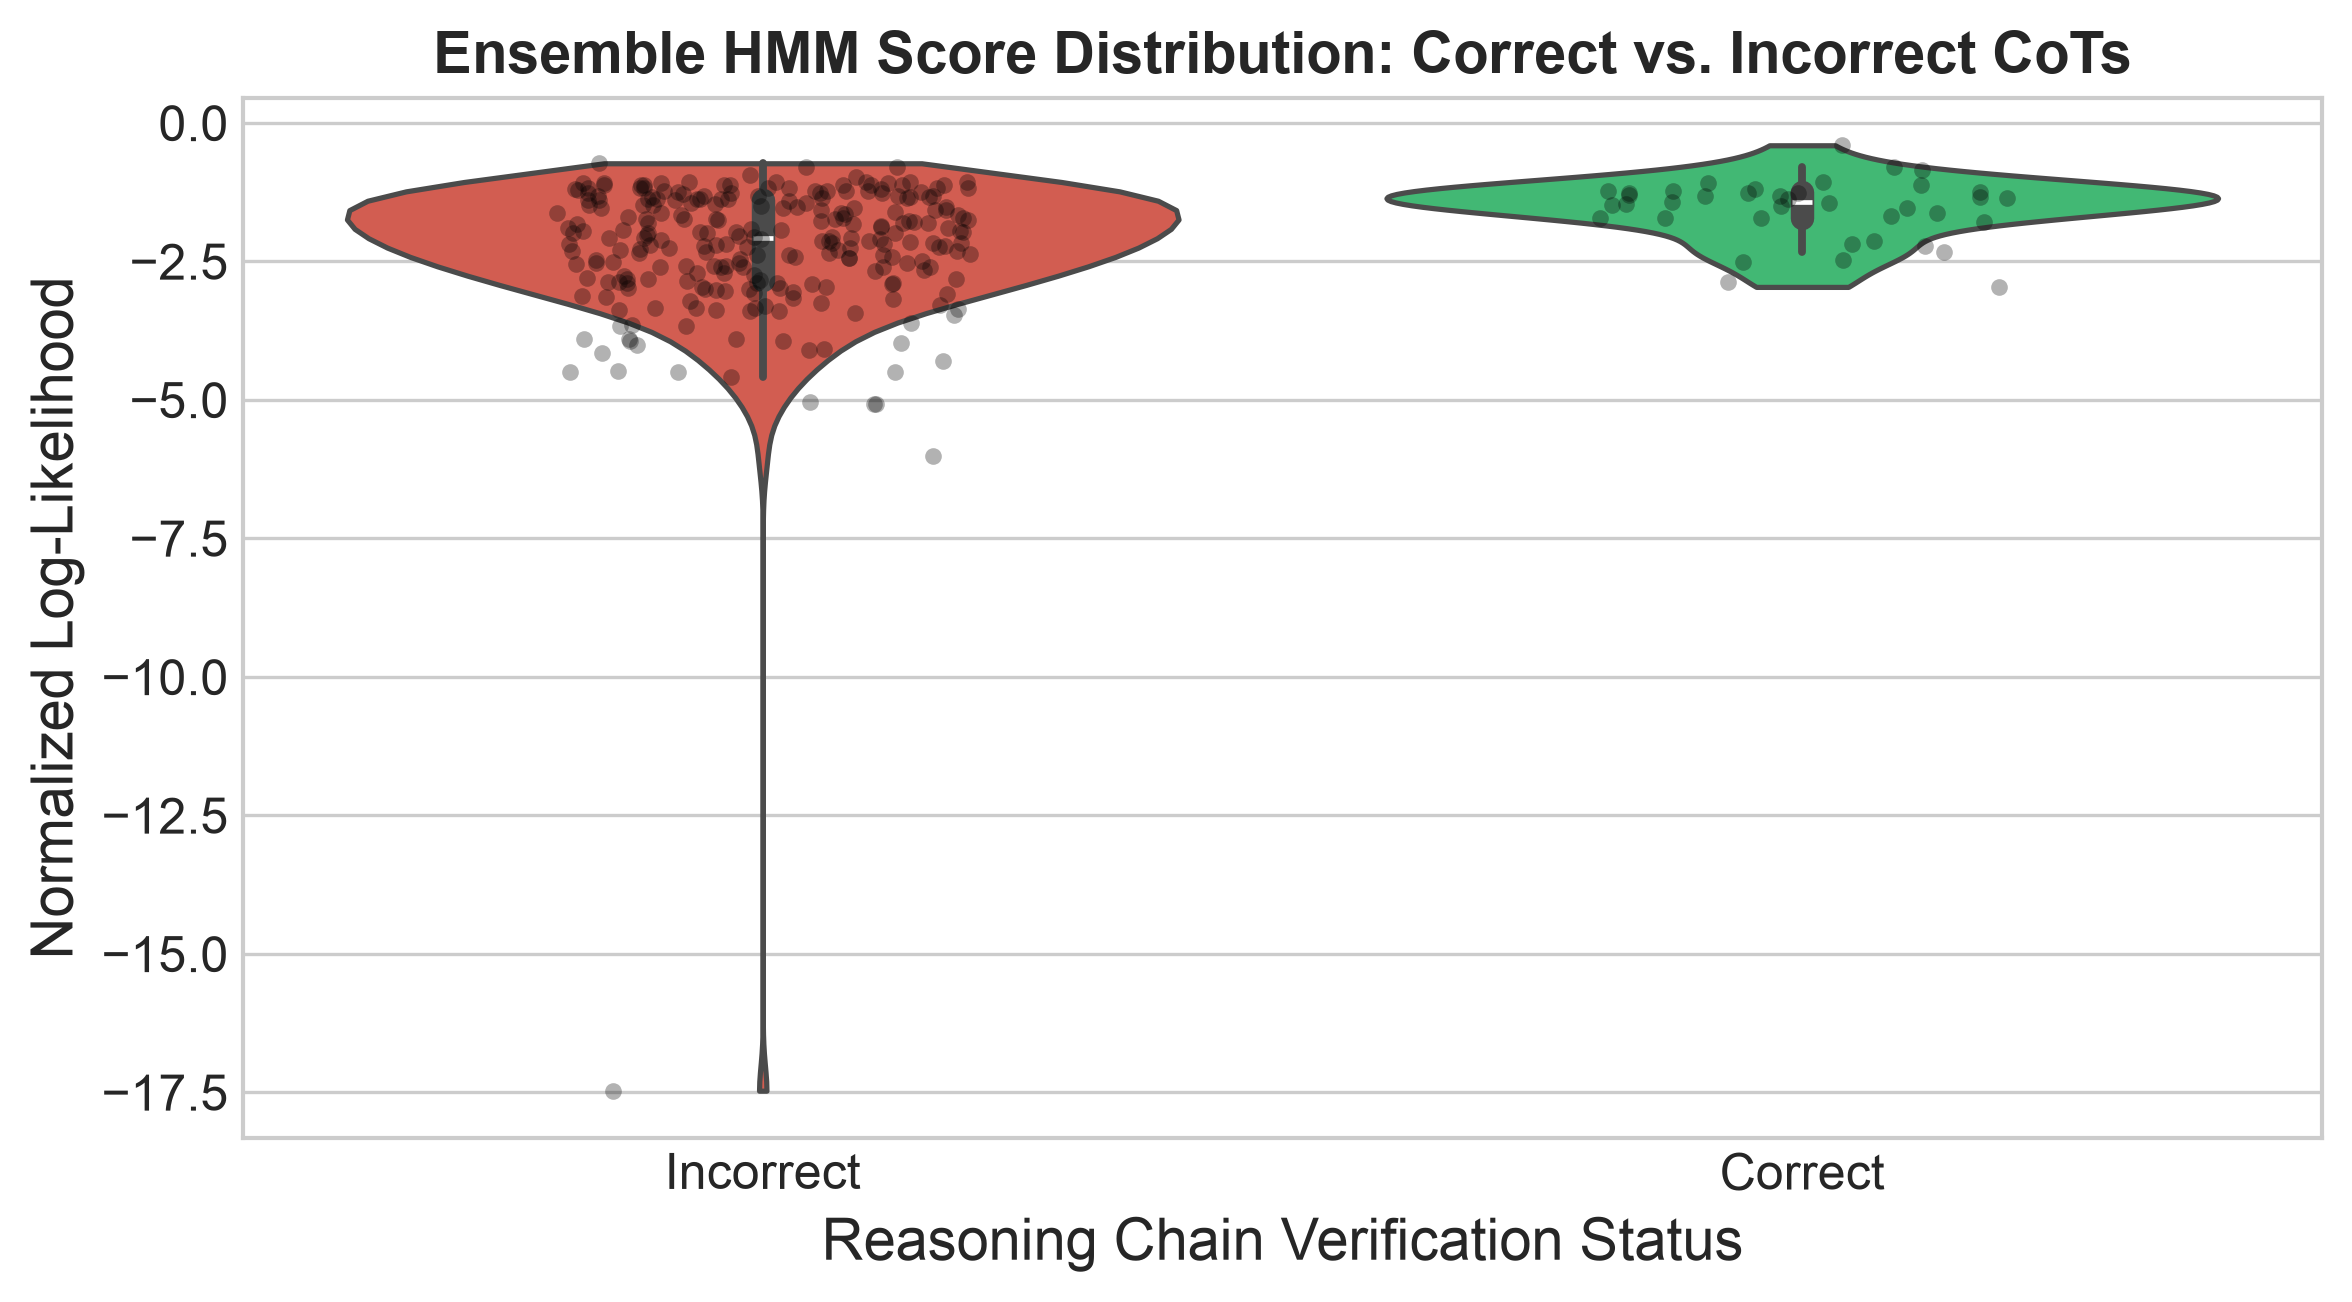
\includegraphics[width=\columnwidth]{figures/fig_distributions.png}}
\caption{Score distributions for Structural HMM vs.\ heuristic baselines: the HMM shows clearer separation between correct and incorrect chains.}
\label{fig:distributions}
\end{figure}

\begin{figure}[htbp]
\centerline{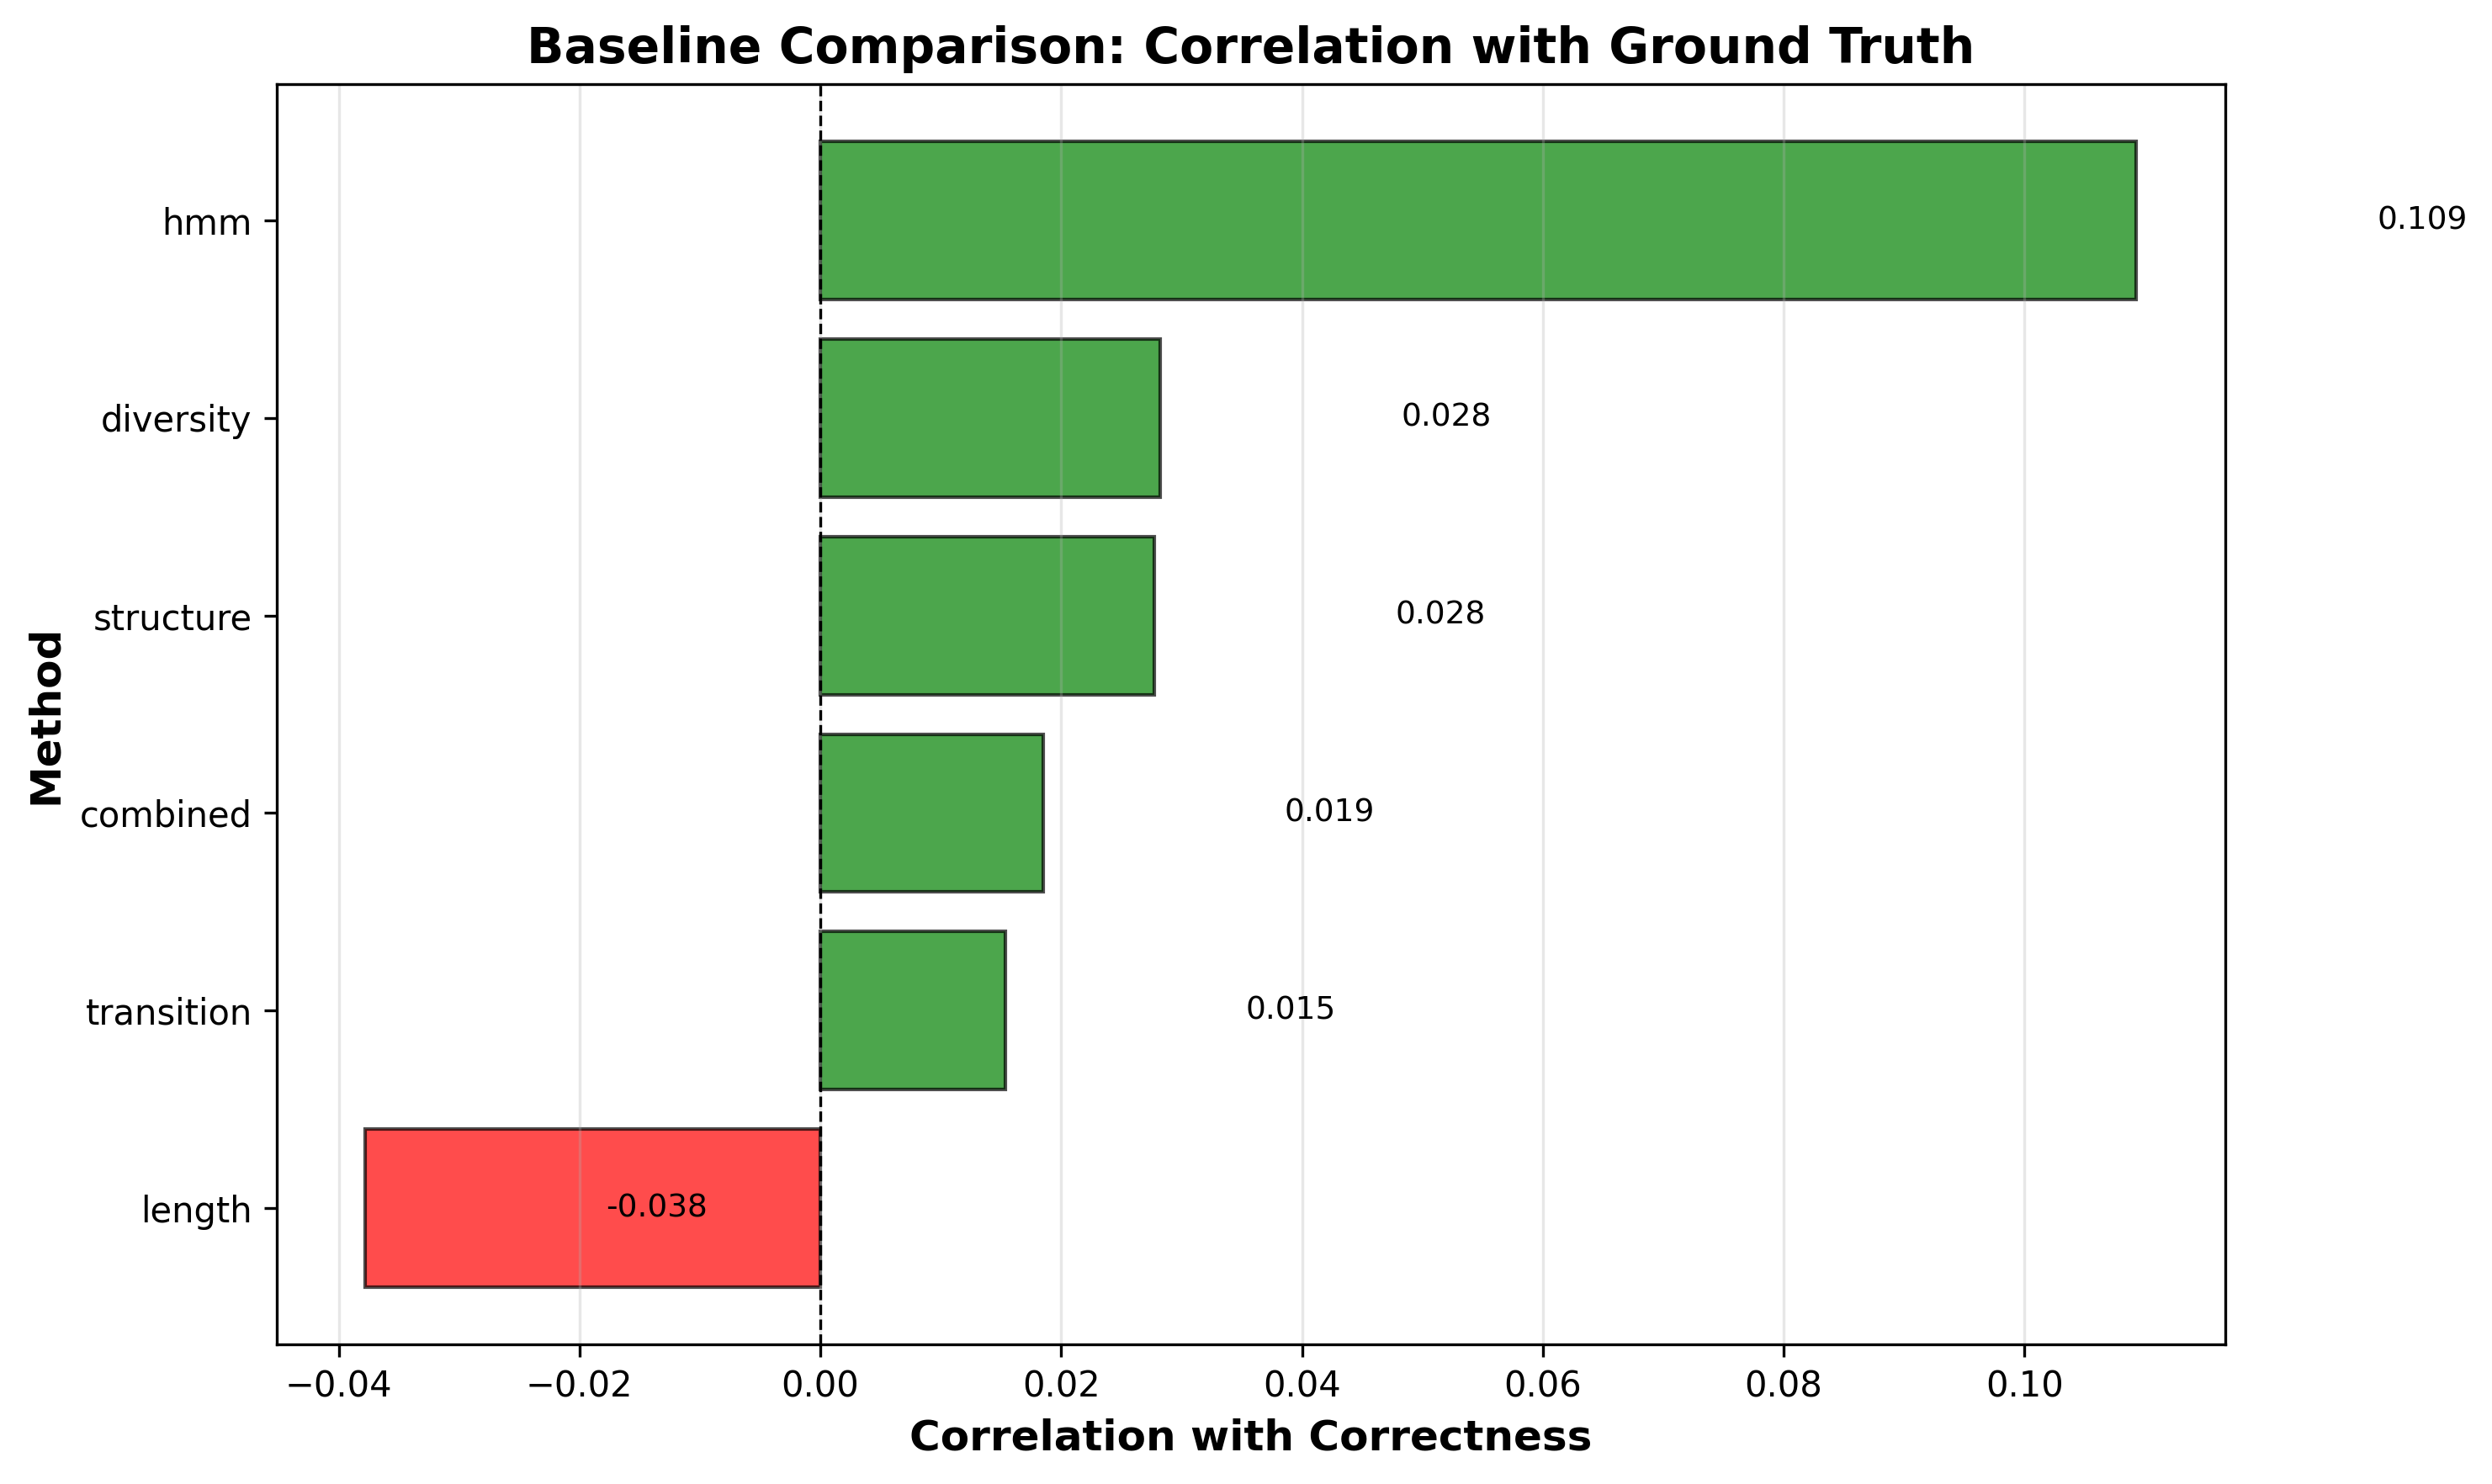
\includegraphics[width=\columnwidth]{figures/fig_correlation.png}}
\caption{Point-biserial correlation comparison: only HMM methods achieve significant positive correlation.}
\label{fig:correlation}
\end{figure}

\begin{figure}[htbp]
\centerline{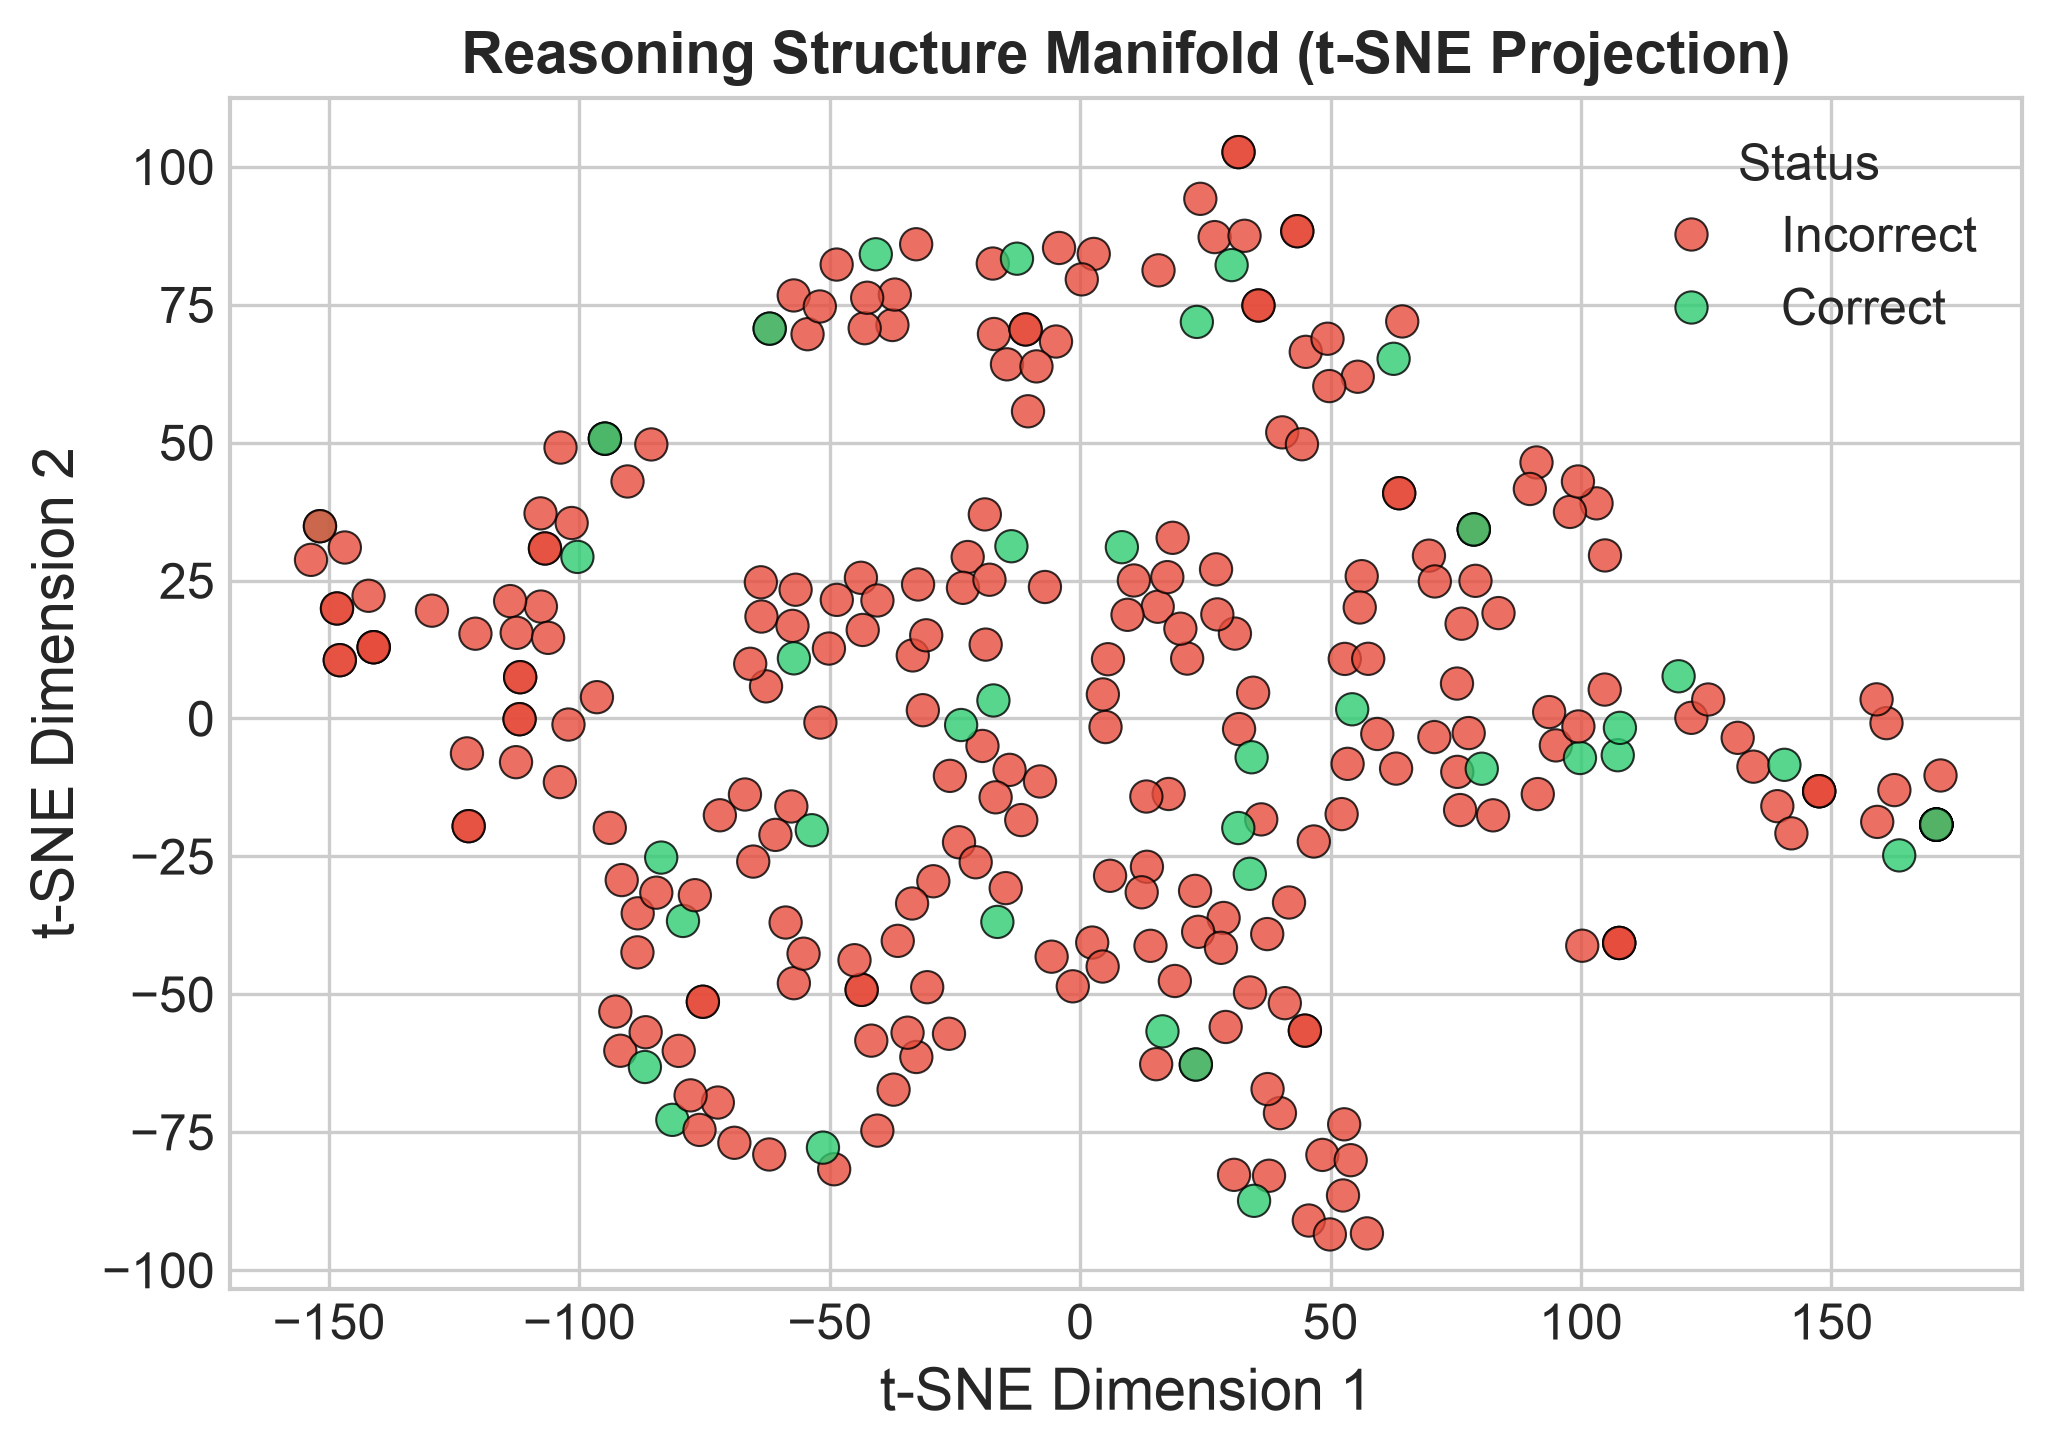
\includegraphics[width=\columnwidth]{figures/reasoning_manifold.png}}
\caption{Reasoning Manifold (t-SNE): correct chains cluster distinctly, while incorrect chains scatter.}
\label{fig:manifold}
\end{figure}

\begin{figure}[htbp]
\centerline{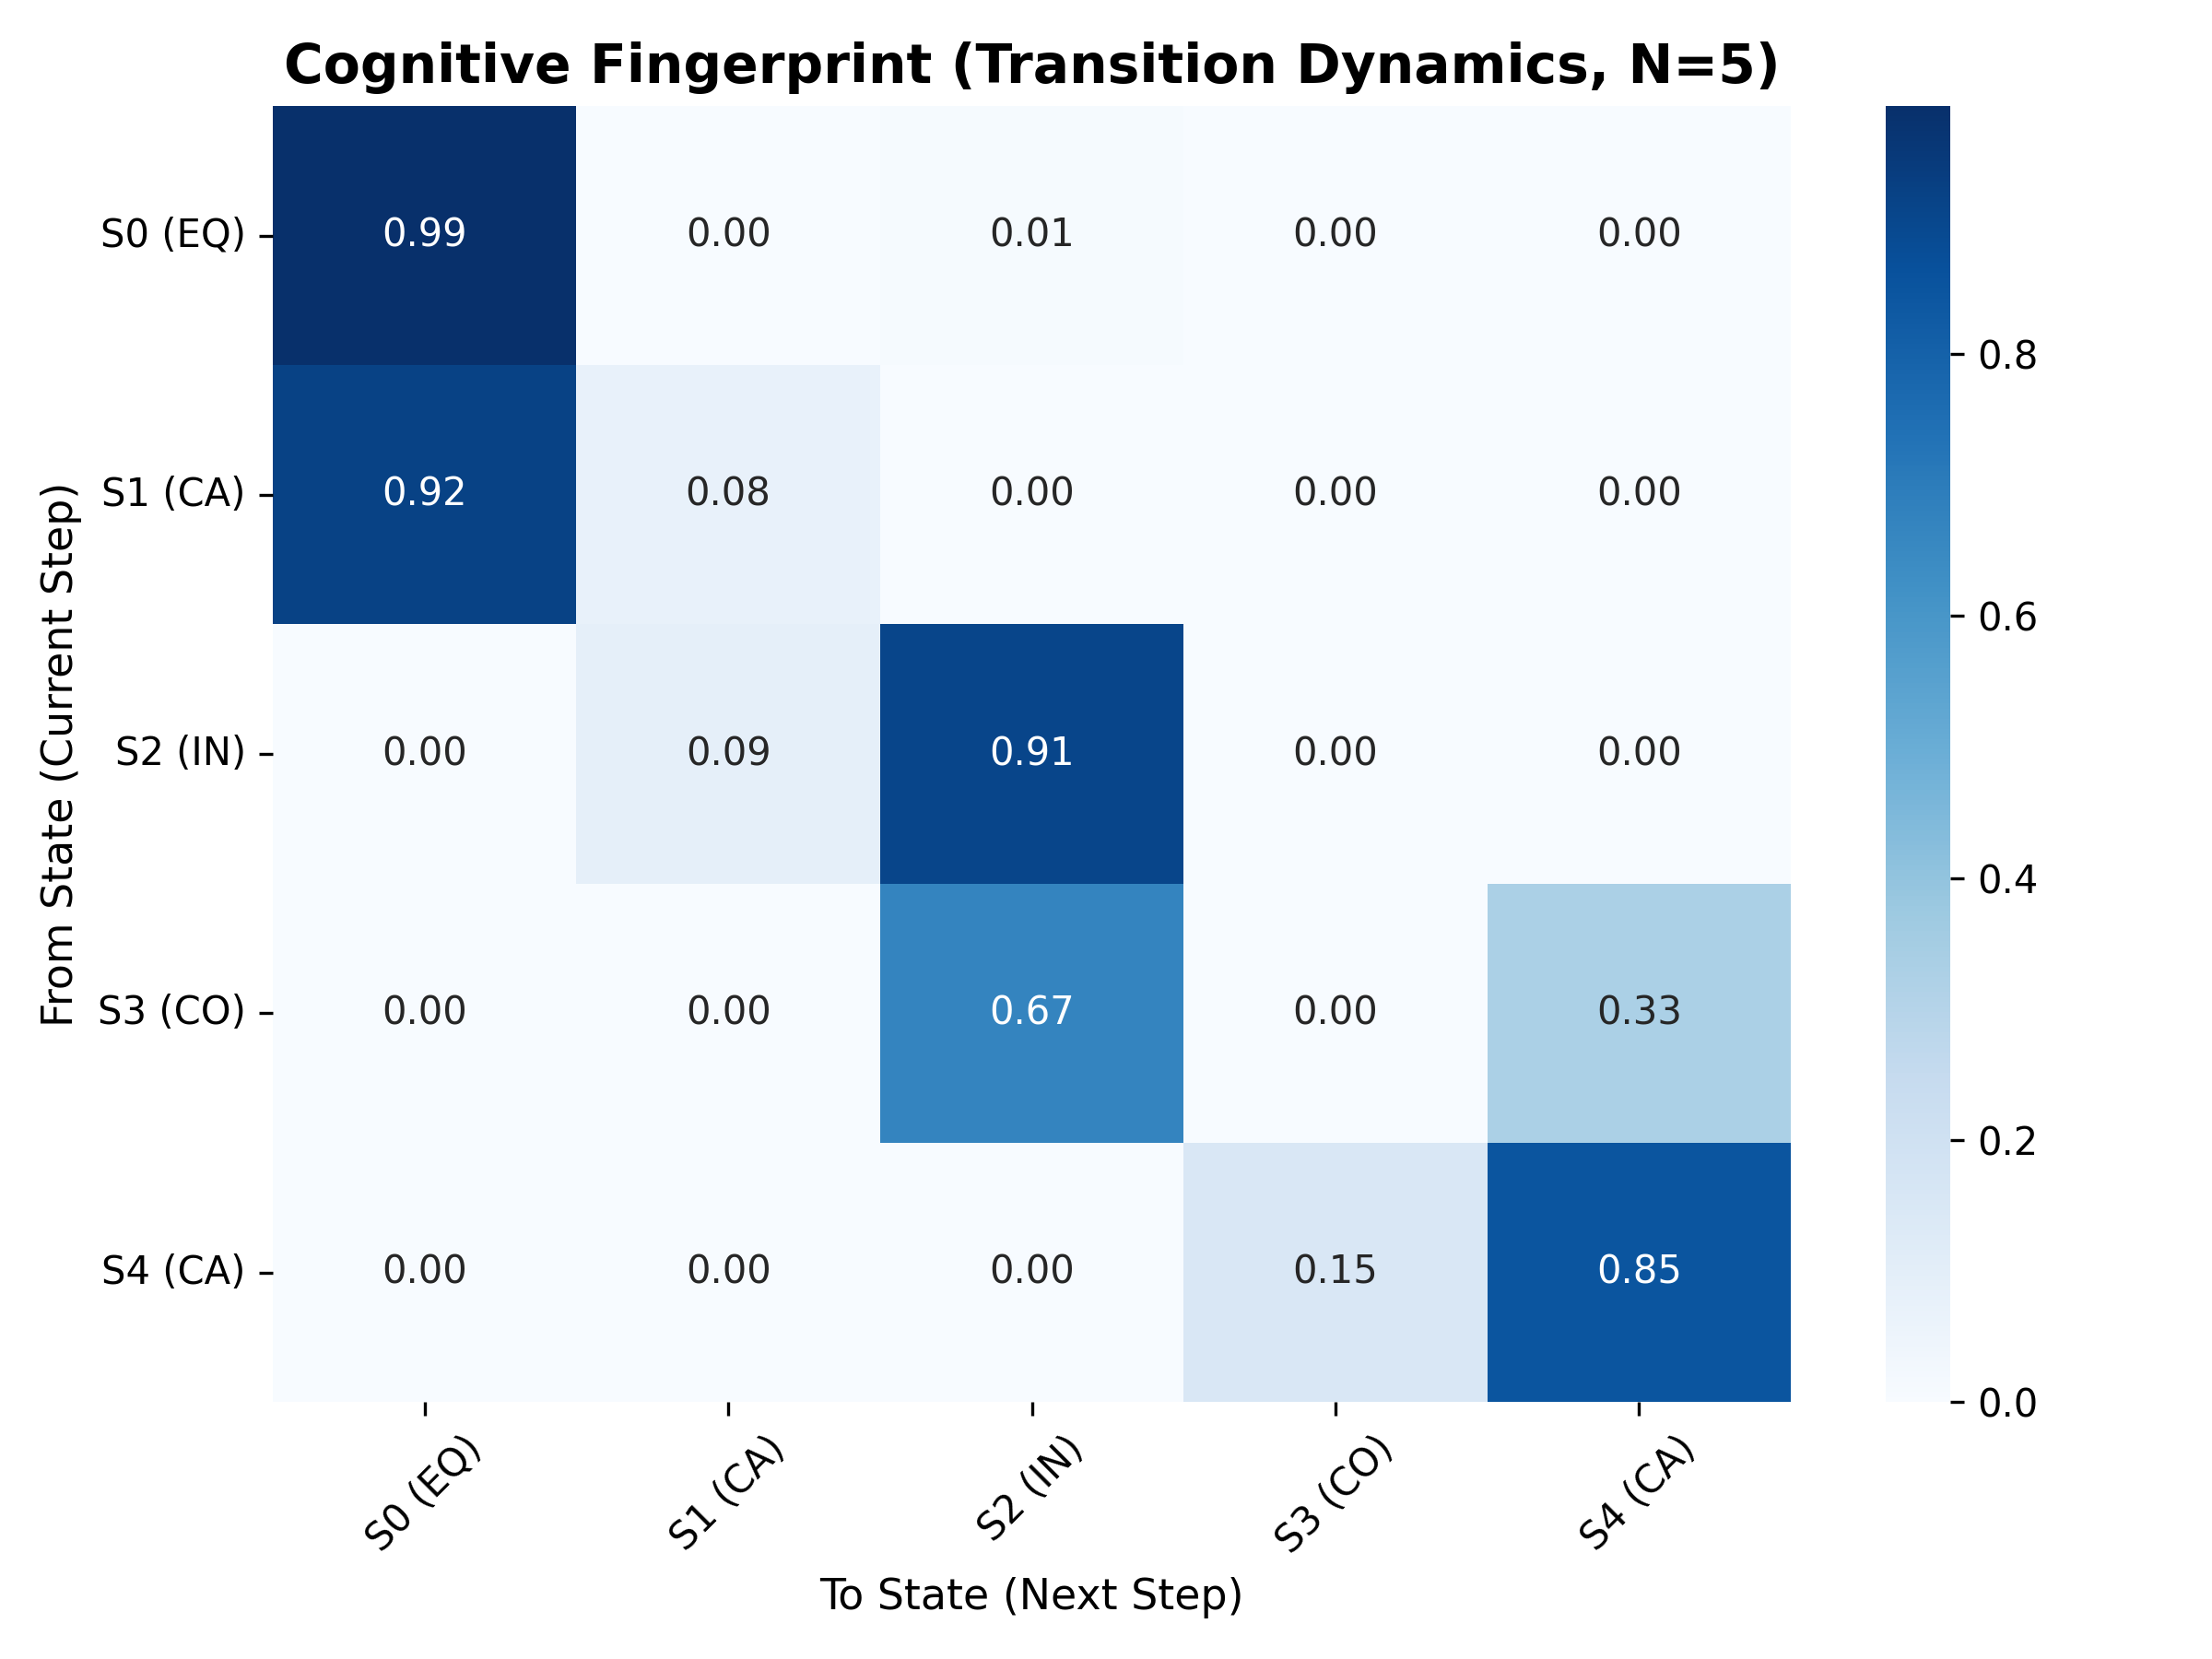
\includegraphics[width=\columnwidth]{figures/cognitive_fingerprint.png}}
\caption{Cognitive Fingerprint: HMM transition matrix heatmap ($N=5$) reveals structured flow (PR$\rightarrow$EQ$\rightarrow$CA$\rightarrow$CO) in correct reasoning.}
\label{fig:fingerprint}
\end{figure}

\begin{figure}[htbp]
\centerline{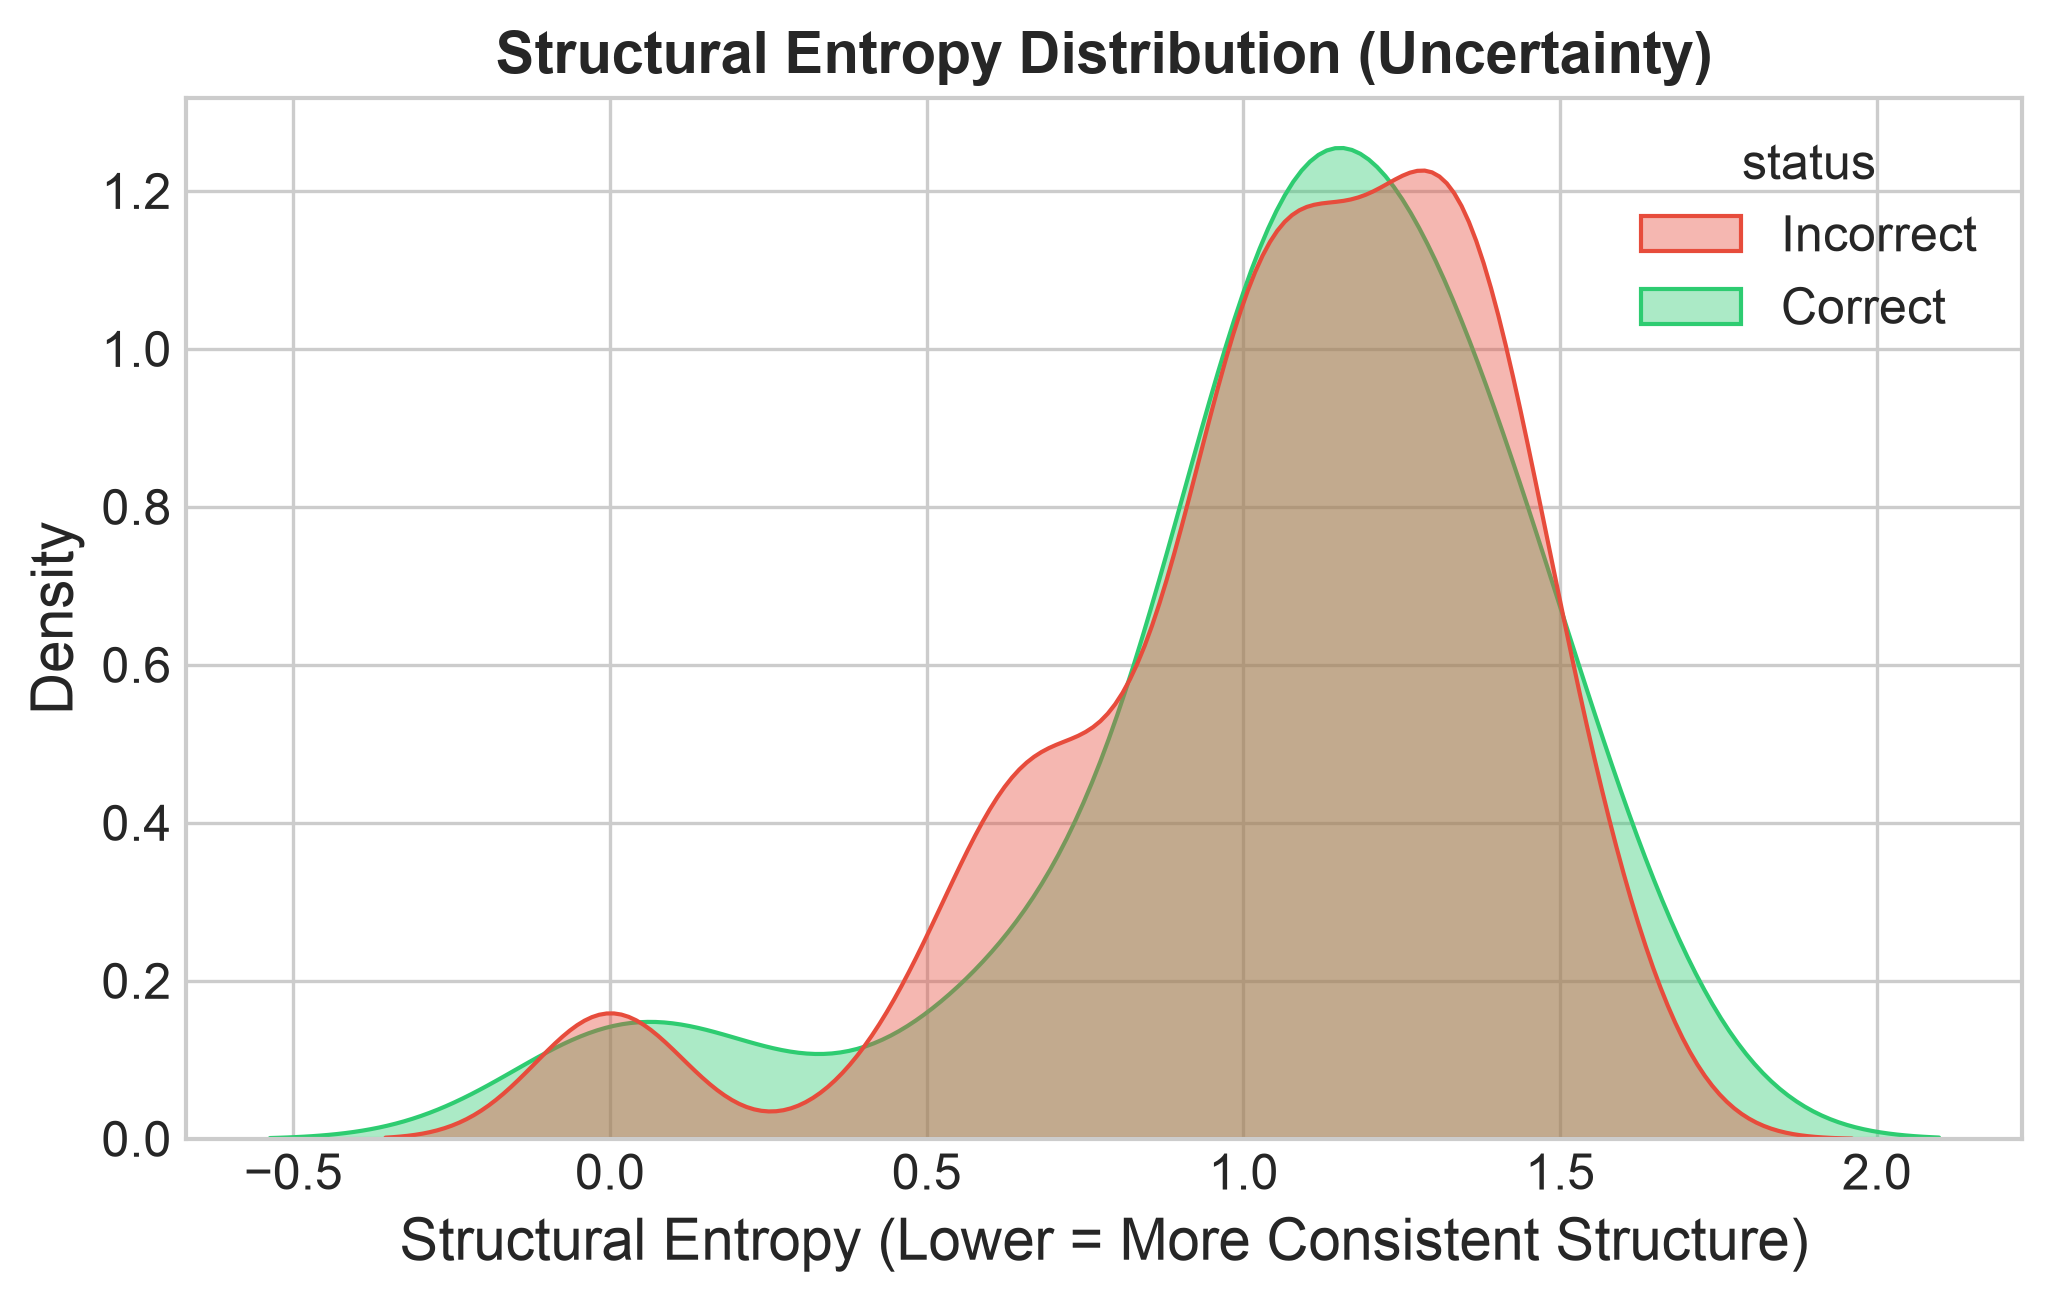
\includegraphics[width=\columnwidth]{figures/structural_entropy.png}}
\caption{Structural Entropy: incorrect chains exhibit significantly higher entropy than correct chains ($p<0.05$ after FDR correction).}
\label{fig:entropy}
\end{figure}

\subsection{Cross-Model, Cross-Domain, and Ablation Results}

Table~\ref{tab:combined} consolidates cross-model, cross-domain, and ablation results. Structural signals scale with model quality: Qwen-1.5B achieves $r=0.25$ vs.\ $r=0.21$ for Qwen-0.5B, suggesting larger models produce more structurally coherent correct reasoning. The HMM shows near-chance performance on ARC science QA even when trained on ARC science QA data ($r\approx0$, AUC$\approx$0.51), as unstructured inference-only tasks lack the discriminative structural patterns present in mathematics. This domain-specificity supports the interpretation that the learned signal captures meaningful task structure rather than generic artifacts.

Figures~\ref{fig:ablation_states} and \ref{fig:ablation_size} show ablation trends. $N=5$ hidden states optimally balances expressiveness and generalization---states naturally align with problem understanding, equation setup, computation, result derivation, and conclusion. For $N{\geq}7$, fragmented state assignments lose interpretability without performance gain. Training data ablation shows substantial improvement from 10 to 50 samples, plateauing beyond 50, enabling data-efficient deployment from small verified-correct corpora.

\begin{figure}[htbp]
\centerline{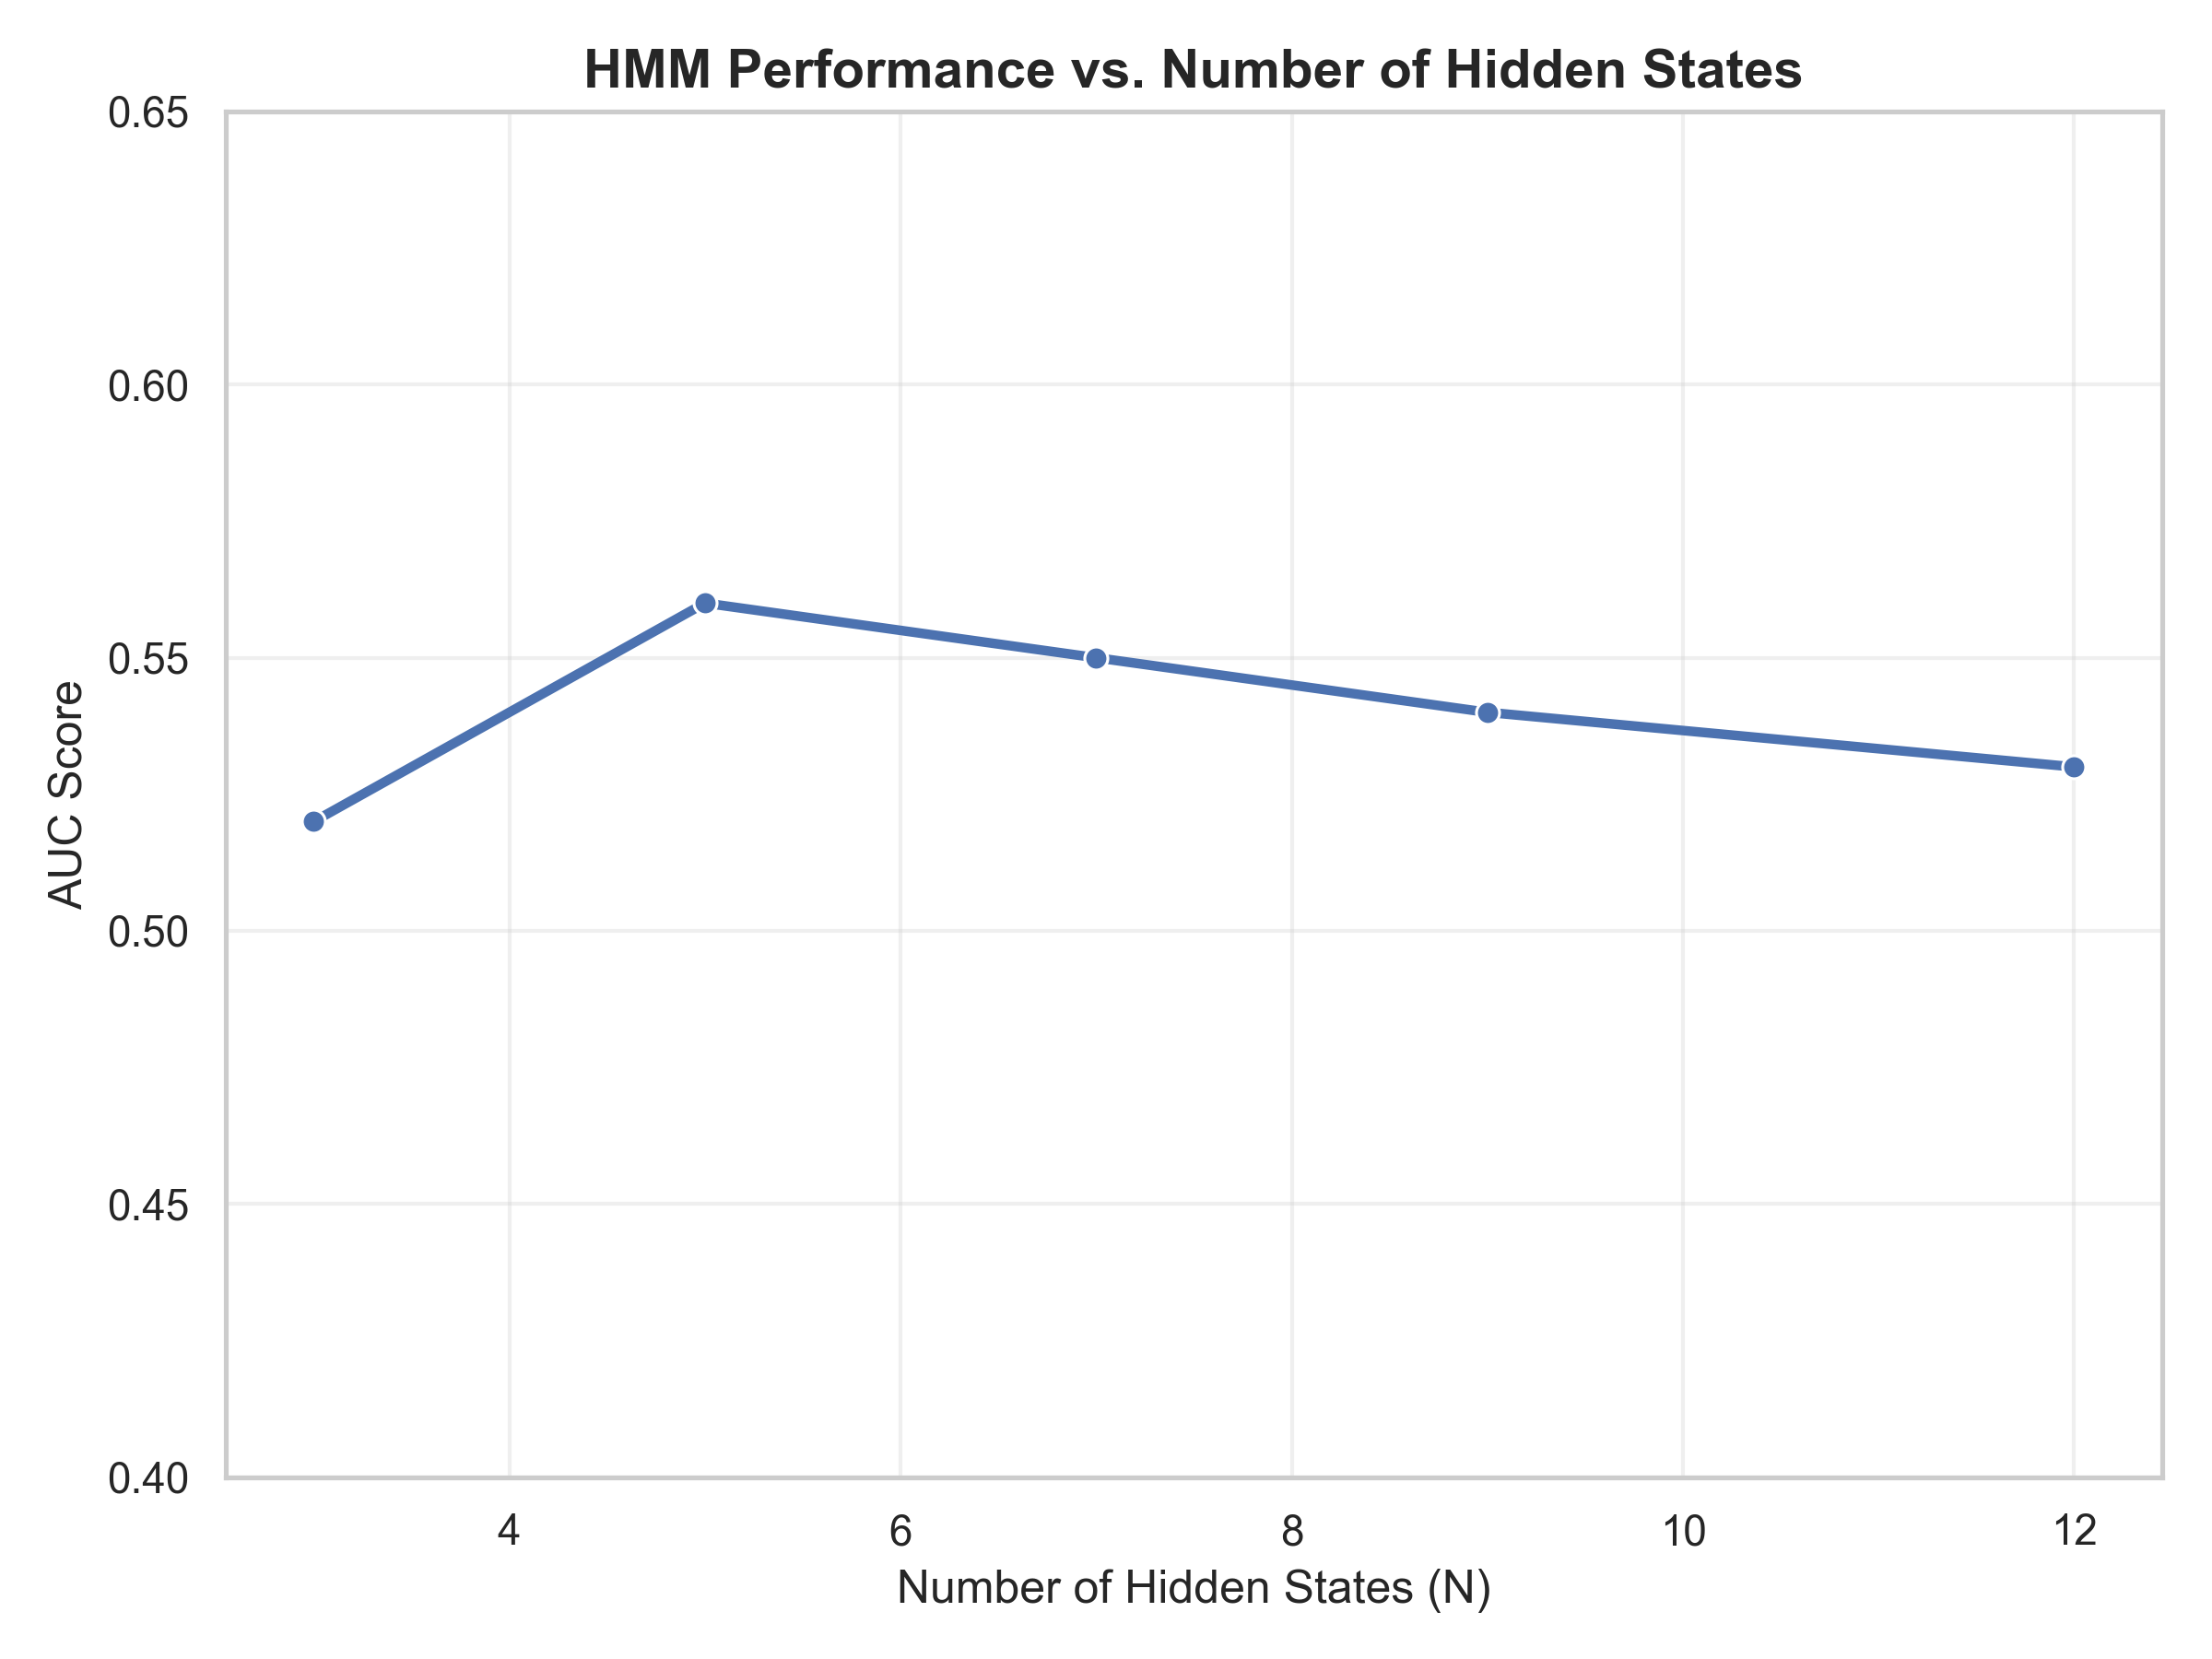
\includegraphics[width=\columnwidth]{figures/fig_ablation_states.png}}
\caption{Ablation: Effect of number of hidden states $N$ on AUC. $N=5$ achieves best balance.}
\label{fig:ablation_states}
\end{figure}

\begin{figure}[htbp]
\centerline{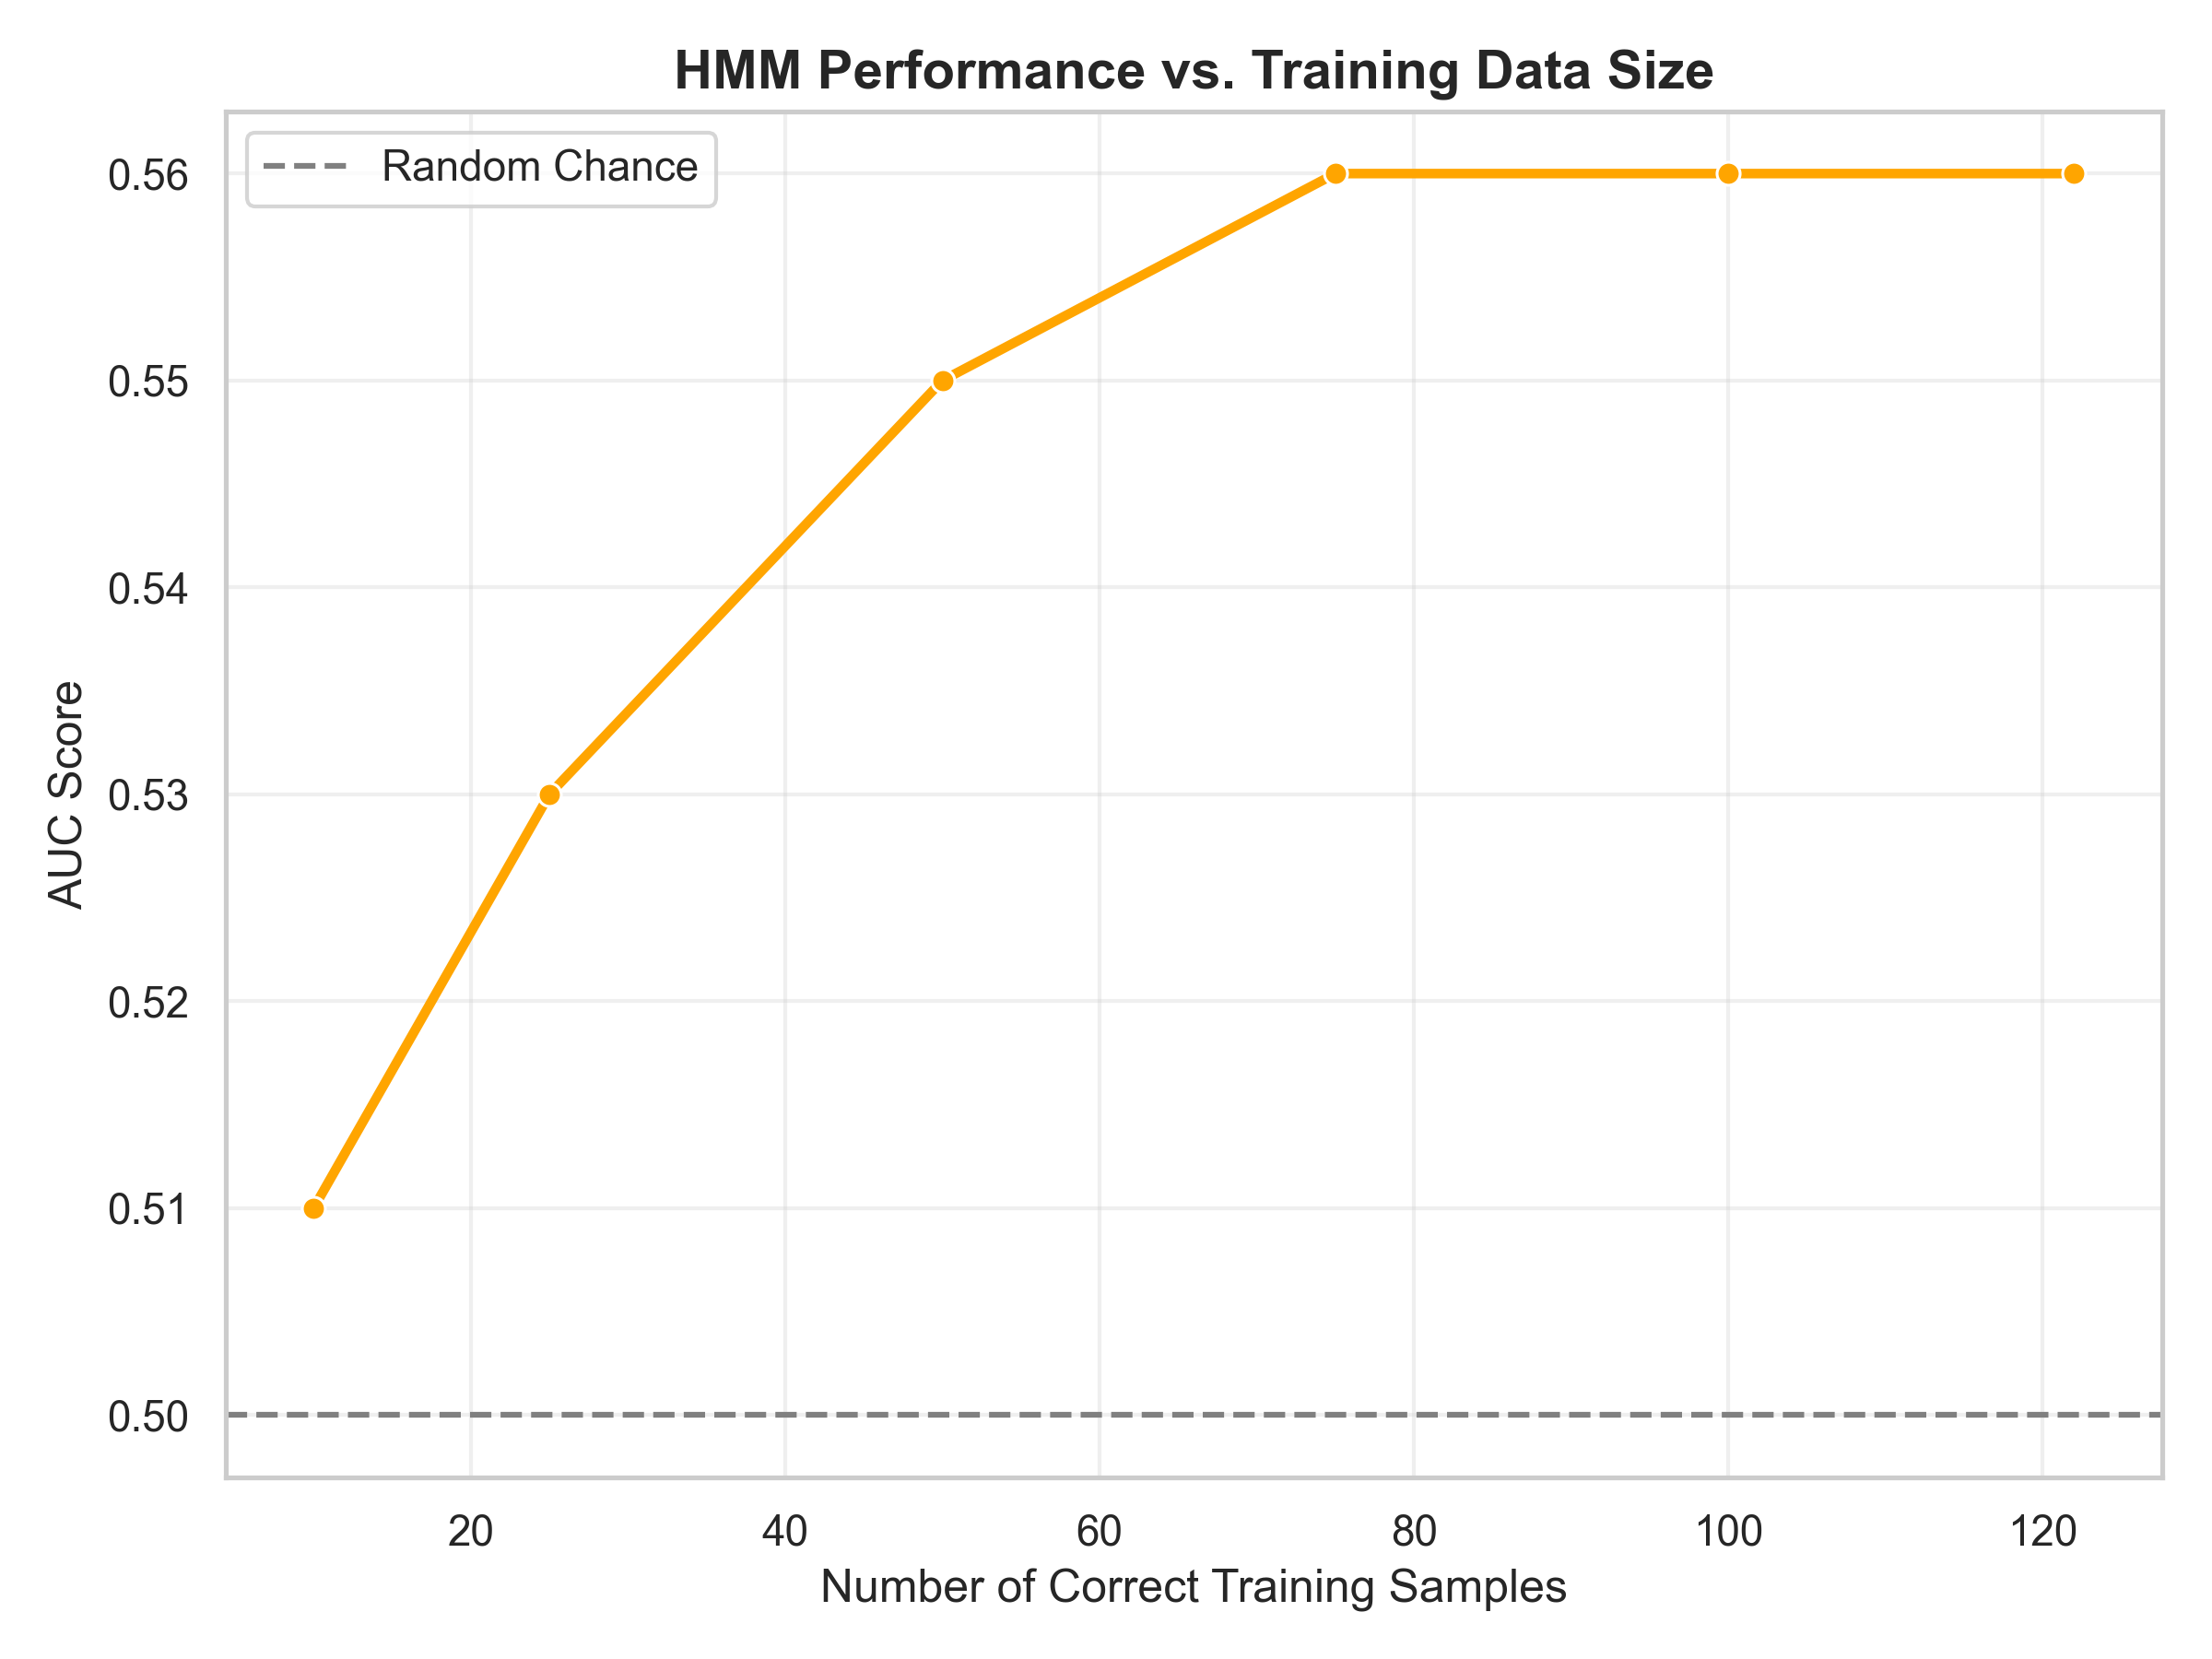
\includegraphics[width=\columnwidth]{figures/fig_ablation_size.png}}
\caption{Ablation: AUC vs.\ training data size. Performance plateaus at 50 correct solutions.}
\label{fig:ablation_size}
\end{figure}

\begin{table}[htbp]
\caption{Consolidated Experimental Results (refer to Fig.~\ref{fig:ablation_size} for full training-size details)}
\label{tab:combined}
\begin{center}
\begin{tabular}{llcc}
\toprule
\textbf{Experiment} & \textbf{Setting} & \textbf{Corr.} & \textbf{AUC} \\
\midrule
\multirow{2}{*}{Cross-Model} & Qwen-0.5B ($N$=150) & 0.21 & 0.62 \\
                              & Qwen-1.5B ($N$=74)  & 0.25 & -- \\
\midrule
\multirow{2}{*}{Cross-Domain} & Math$\rightarrow$Science & 0.04 & 0.46 \\
                               & Science$\rightarrow$Science & 0.02 & 0.51 \\
\midrule
\multirow{5}{*}{Hidden States $N$} & 3 & -- & 0.52 \\
 & 5 (best) & -- & 0.56 \\
 & 7 & -- & 0.55 \\
 & 9 & -- & 0.54 \\
 & 12 & -- & 0.53 \\
\midrule
\multirow{3}{*}{Train Size} & 10 & -- & 0.51 \\
 & 50 & -- & 0.55 \\
 & 122 (full) & -- & 0.56 \\
\bottomrule
\end{tabular}
\end{center}
\end{table}

\subsection{Qualitative Analysis}

Figure~\ref{fig:transition} shows learned transition matrices. \textbf{Correct chains} follow structured progressions (PR$\rightarrow$EQ$\rightarrow$CA$\rightarrow$CO), reflecting organized problem-solving. \textbf{Incorrect chains} show anomalous patterns:
\begin{itemize}
    \item Premature conclusions: CO appearing early without supporting CA steps.
    \item Missing computations: PR$\rightarrow$IN$\rightarrow$CO without CA.
    \item Circular reasoning: extended loops of IN$\rightarrow$IN or CA$\rightarrow$EQ$\rightarrow$CA$\rightarrow$EQ.
    \item Diversions: DV tags indicating off-topic or confused logic.
\end{itemize}
Statistically, 77.8\% of looping solutions ($N$=150) were incorrect vs.\ only 23.8\% of non-looping ones, a highly significant difference ($z=6.18$, $p=6.3{\times}10^{-10}$).

\begin{figure}[htbp]
\centerline{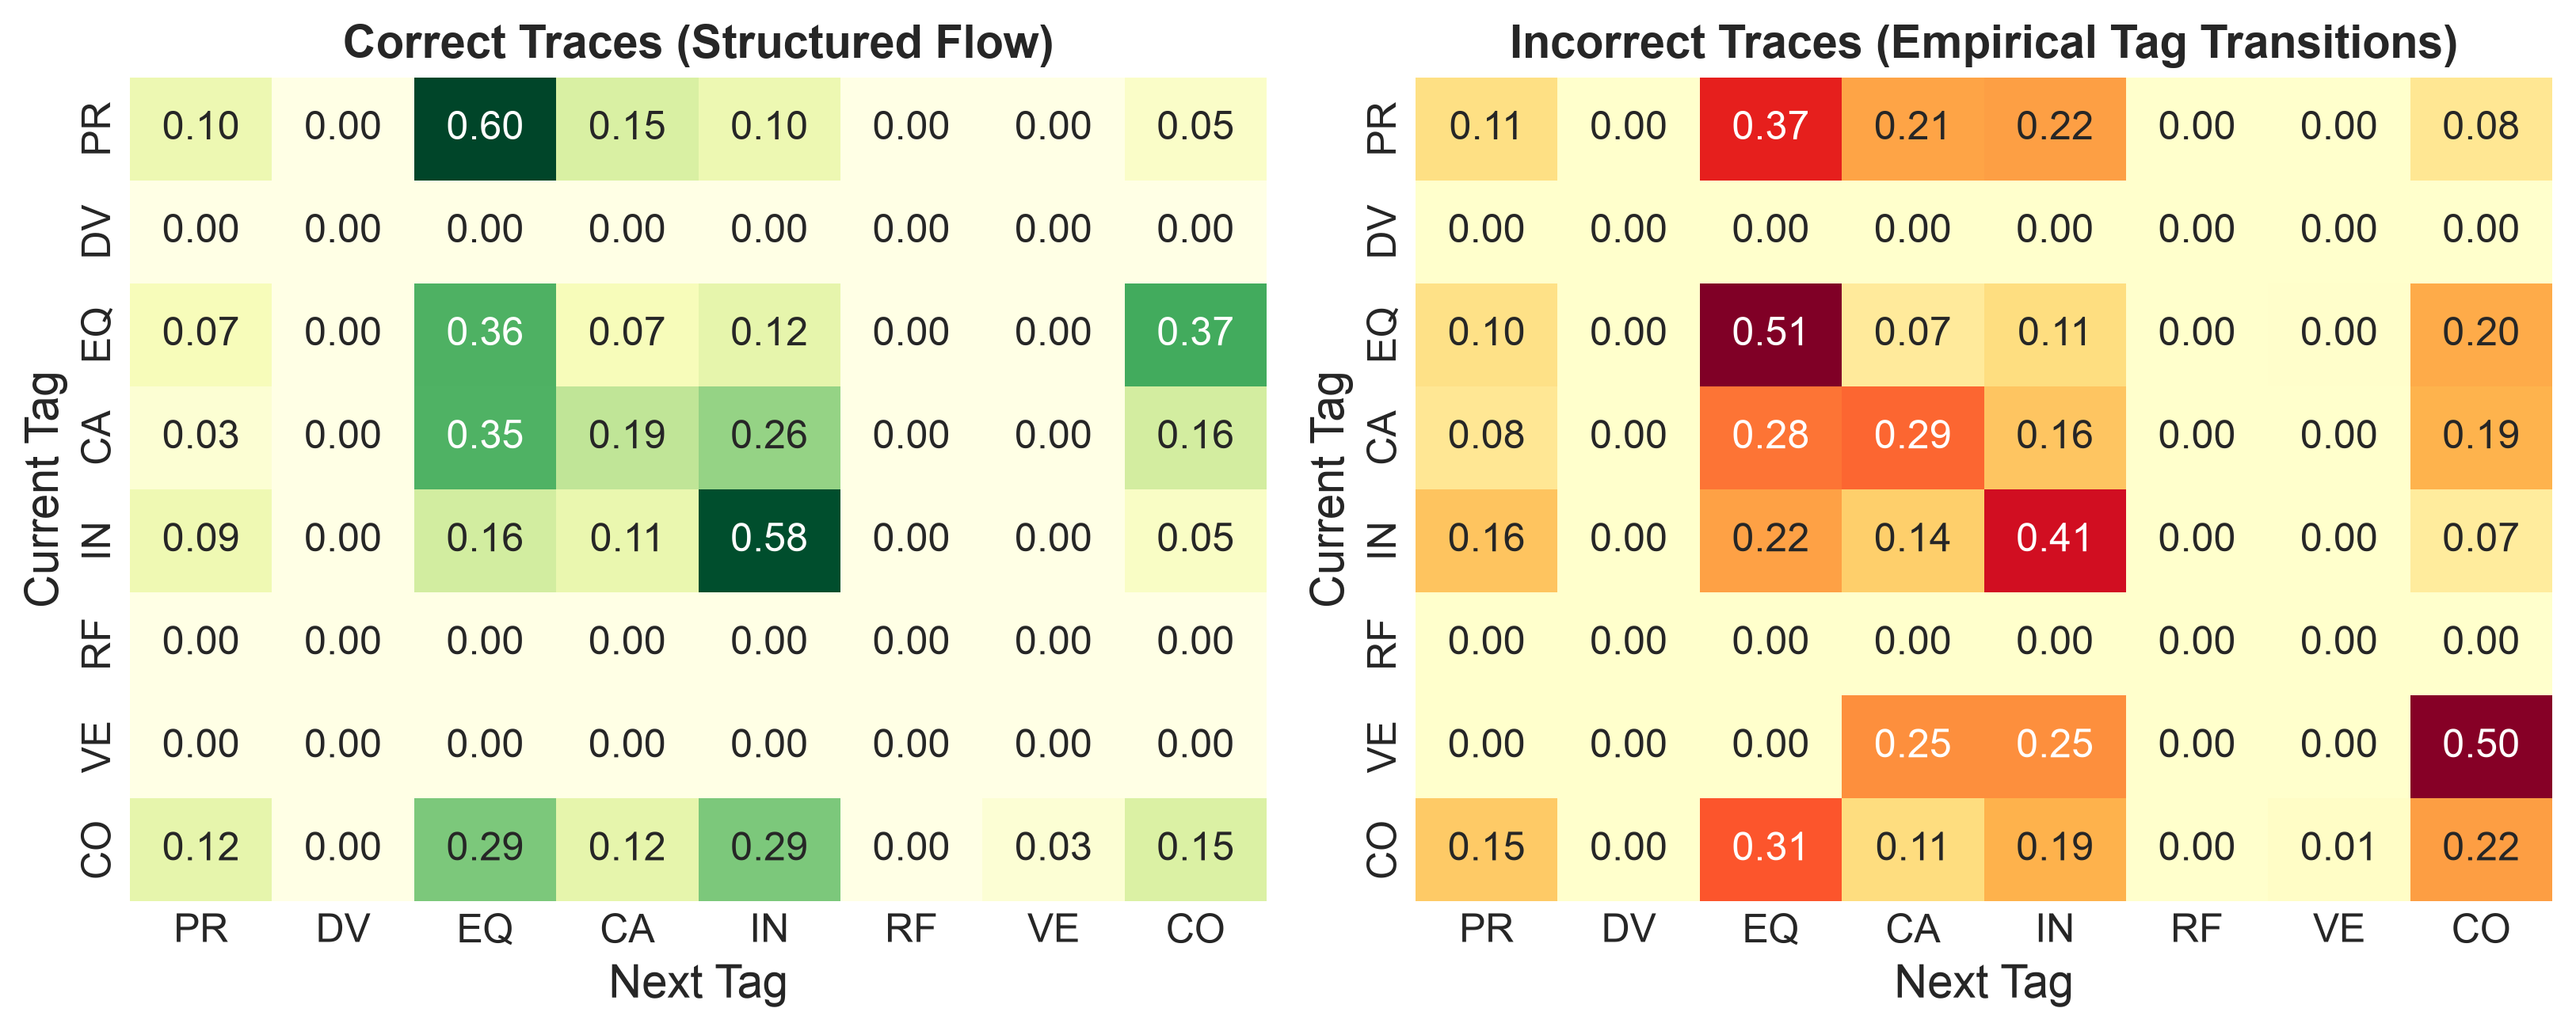
\includegraphics[width=\columnwidth]{figures/fig_transition.png}}
\caption{Transition matrices: Correct chains show structured PR$\rightarrow$EQ$\rightarrow$CA flow; incorrect chains show chaotic transitions and loops.}
\label{fig:transition}
\end{figure}

Representative cases: A \textit{true positive} (score $-1.49$, tag sequence [PR, IN, CA, IN, CA, CO]) follows a clean setup$\rightarrow$compute$\rightarrow$conclude pattern. A \textit{false positive} (score $-1.38$, [CA, IN, CA, CO]) appears structurally valid but contains arithmetic errors---the core ``Structural Hallucination'' failure mode. A \textit{true negative} (score $-4.59$, [DV, RF, CA, CA, CO]) is correctly flagged by initial Diversion and Reflection tags. Rare \textit{false negatives} occur for conclusion-first reasoning patterns underrepresented in training data.

\section{Discussion and Conclusion}

\textbf{Practical Applications.} Low structural scores can trigger \textit{rejection sampling}, filtering likely errors before expensive semantic verification. Aggregate structural statistics enable \textit{quality monitoring} without ground-truth answers, and structural anomalies serve as a \textit{debugging aid} for reviewers.

\textbf{Why Structure Matters.} Human problem-solving follows characteristic phases; LLMs trained on human data internalize these patterns. Many reasoning errors---skipped steps, circular arguments, premature conclusions---manifest structurally even when individual steps appear semantically plausible. For instance, in mathematical reasoning, a common error manifests as skipping necessary arithmetic calculations (a missing CA tag) or stating a conclusion immediately after problem restatement (a direct PR$\rightarrow$CO transition).

\textbf{Limitations.} (1) \textit{Structural Hallucinations}: well-structured but semantically wrong chains receive high scores---structure is necessary but not sufficient. (2) \textit{Domain Specificity}: separate models are needed per reasoning domain. (3) \textit{Sample Size}: larger-scale evaluation would strengthen findings. Future research directions include: (1) investigating neural-HMM hybrids that use neural networks to parameterize emission distributions; (2) exploring multi-domain mixture models to address cross-domain transfer; and (3) integrating structural scores with token-level PRMs for a combined verification system.

\textbf{Conclusion.} We introduced an unsupervised, lightweight CoT verification method based on Ensemble HMMs over semantic tag sequences. Key contributions:
\begin{itemize}
    \item \textbf{Ensemble HMMs:} A diverse jury of $M=12$ models with varying state complexities doubled the point-biserial correlation ($r\!:\!0.11{\to}0.21$, $p<0.01$) over single-model HMM baselines.
    \item \textbf{Structural Entropy:} A novel structural uncertainty metric showing significantly lower entropy in correct reasoning chains ($p<0.05$).
    \item \textbf{Visual Interpretability:} Reasoning Manifolds and Cognitive Fingerprints provide visual evidence that correctness exhibits structural patterns.
    \item \textbf{Robustness and Specificity:} Difficulty-invariance ($r=0.04$ with length) and domain-specificity (near-chance performance on ARC science QA) support the interpretation that the method captures task-specific patterns.
\end{itemize}
Running at milliseconds per sample with no labeling requirement, our method offers a practical first-line verification filter, and the \texttt{StructureReward} class is exposed as future-facing infrastructure for reinforcement learning pipelines.

\begin{thebibliography}{00}
\bibitem{wei2022chain} J. Wei et al., ``Chain-of-thought prompting elicits reasoning in large language models,'' in \textit{Proc. NeurIPS}, vol. 35, 2022, pp. 24824--24837.

\bibitem{ji2023survey} Z. Ji et al., ``Survey of hallucination in natural language generation,'' \textit{ACM Comput. Surv.}, vol. 55, no. 12, pp. 1--38, 2023.

\bibitem{lightman2024let} H. Lightman et al., ``Let's verify step by step,'' in \textit{Proc. ICLR}, 2024.

\bibitem{wang2023self} X. Wang et al., ``Self-consistency improves chain of thought reasoning in language models,'' in \textit{Proc. ICLR}, 2023.

\bibitem{kojima2022large} T. Kojima, S. S. Gu, M. Reid, Y. Matsuo, and Y. Iwasawa, ``Large language models are zero-shot reasoners,'' in \textit{Proc. NeurIPS}, vol. 35, 2022, pp. 22199--22213.

\bibitem{zhou2023least} D. Zhou et al., ``Least-to-most prompting enables complex reasoning in large language models,'' in \textit{Proc. ICLR}, 2023.

\bibitem{yao2023tree} S. Yao, D. Yu, J. Zhao, I. Shafran, T. Griffiths, Y. Cao, and K. Narasimhan, ``Tree of thoughts: Deliberate problem solving with large language models,'' in \textit{Proc. NeurIPS}, vol. 36, 2023, pp. 11809--11822.

\bibitem{weng2023large} Y. Weng, W. Zhu, F. Xia, M. Zhu, S. He, and K. Liu, ``Large language models are better reasoners with self-verification,'' in \textit{Proc. EMNLP Findings}, 2023, pp. 2550--2575.

\bibitem{rabiner1989tutorial} L. R. Rabiner, ``A tutorial on hidden Markov models and selected applications in speech recognition,'' \textit{Proc. IEEE}, vol. 77, no. 2, pp. 257--286, 1989.

\bibitem{wiseman2018learning} S. Wiseman, S. Rush, S. Shieber, and J. Kim, ``Learning neural templates for text generation,'' in \textit{Proc. EMNLP}, 2018, pp. 3174--3187.

\bibitem{lcot2tree2025} G. Jiang et al., ``What makes a good reasoning chain? Uncovering structural patterns in long chain-of-thought reasoning,'' \textit{arXiv preprint arXiv:2501.09000}, 2025.

\bibitem{picsar2025} J. O. J. Leang et al., ``PiCSAR: Probabilistic Confidence Selection And Ranking for Reasoning Chains,'' \textit{arXiv preprint arXiv:2501.08000}, 2025.

\bibitem{zhang2020bertscore} T. Zhang, V. Kishore, F. Wu, K. Q. Weinberger, and Y. Artzi, ``BERTScore: Evaluating text generation with BERT,'' in \textit{Proc. ICLR}, 2020.

\bibitem{golovneva2023roscoe} O. Golovneva et al., ``ROSCOE: A suite of metrics for scoring step-by-step reasoning,'' in \textit{Proc. ICLR}, 2023.

\bibitem{wang-etal-2024-math-shepherd} P. Wang et al., ``Math-Shepherd: Verify and Reinforce LLMs Step-by-step without Human Annotations,'' in \textit{Proc. ACL}, 2024, pp. 9306--9318.

\bibitem{khalifa2025} M. Khalifa, A. G. G. de Oliveira, and E. X. Wu, ``Process Reward Models That Think,'' \textit{arXiv preprint arXiv:2504.16828}, 2025.

\bibitem{cobbe2021training} K. Cobbe et al., ``Training verifiers to solve math word problems,'' \textit{arXiv preprint arXiv:2110.14168}, 2021.

\bibitem{clark2018think} P. Clark et al., ``Think you have solved question answering? Try ARC,'' \textit{arXiv preprint arXiv:1803.05457}, 2018.

\bibitem{landis1977measurement} J. R. Landis and G. G. Koch, ``The measurement of observer agreement for categorical data,'' \textit{Biometrics}, vol. 33, no. 1, pp. 159--174, 1977.
\end{thebibliography}

\end{document}
